% advsync/rt.tex
% mainfile: ../perfbook.tex
% SPDX-License-Identifier: CC-BY-SA-3.0

\section{Parallel Real-Time Computing}
\label{sec:advsync:Parallel Real-Time Computing}
%
\epigraph{One always has time enough if one applies it well.}
	 {\emph{Johann Wolfgang von G\"othe}}
% \epigraph{The difference between you and me is that I was right in time.}
% 	 {\emph{Konrad Adenauer}}
% No support for this quote found.

컴퓨팅에서 중요한 발전중인 분야는 병렬 리얼타임 컴퓨팅입니다.
\Cref{sec:advsync:What is Real-Time Computing?}
는 ``리얼타임 컴퓨팅'' 의 여러 정의를 알아봐서 일반적인 느낌이 아닌 의미 있는
기준으로 넘어갑니다.
\Cref{sec:advsync:Who Needs Real-Time?}
는 리얼타임 응답이 필요한 어플리케이션의 종류를 알아봅니다.
\Cref{sec:advsync:Who Needs Parallel Real-Time?}
는 병렬 리얼타임 컴퓨팅이 우리 곁에 있음을 알리고 언제 그리고 왜 병렬 리얼타임
컴퓨팅이 유용한지 이야기 합니다.
\Cref{sec:advsync:Implementing Parallel Real-Time Systems}
는 병렬 리얼타임 시스템이 어떻게 구현될 수 있는지 간단한 개론을 제공하며,
\cref{sec:advsync:Implementing Parallel Real-Time Operating Systems,%
sec:advsync:Implementing Parallel Real-Time Applications}
는 운영체제와 어플리케이션에 각각 집중합니다.
마지막으로,
\cref{sec:advsync:Real Time vs. Real Fast: How to Choose?}
는 여러분의 어플리케이션이 리얼타임 기능을 필요로 하는지를 어떻게 결정하는지
설명합니다.

\iffalse

An important emerging area in computing is that of parallel real-time
computing.
\Cref{sec:advsync:What is Real-Time Computing?}
looks at a number of definitions of ``real-time computing'', moving
beyond the usual sound bites to more meaningful criteria.
\Cref{sec:advsync:Who Needs Real-Time?}
surveys the sorts of applications that need real-time response.
\Cref{sec:advsync:Who Needs Parallel Real-Time?}
notes that parallel real-time computing is upon us, and discusses
when and why parallel real-time computing can be useful.
\Cref{sec:advsync:Implementing Parallel Real-Time Systems}
gives a brief overview of how parallel real-time systems may be implemented,
with
\cref{sec:advsync:Implementing Parallel Real-Time Operating Systems,%
sec:advsync:Implementing Parallel Real-Time Applications}
focusing on operating systems and applications, respectively.
Finally,
\cref{sec:advsync:Real Time vs. Real Fast: How to Choose?}
outlines how to decide whether or not your application needs real-time
facilities.

\fi

\subsection{What is Real-Time Computing?}
\label{sec:advsync:What is Real-Time Computing?}

리얼타임 컴퓨팅을 분류하는 한가지 전통적 방법은 \emph{하드 리얼타임} 과
\emph{소프트 리얼타임} 으로 카테고리를 나누는 것으로, 하드 리얼타임
어플리케이션은 기한을 결코 어기지 않지만 소프트 리얼타임 어플리케이션은 꽤 자주
기한을 어길 수 있습니다.

\iffalse

One traditional way of classifying real-time computing is into the
categories of \emph{hard real time} and \emph{soft real time}, where
the macho hard real-time applications never miss their deadlines, but
the wimpy soft real-time applications miss their deadlines quite often.

\fi

\subsubsection{Soft Real Time}
\label{sec:Soft Real Time}

이 소프트 리얼타임의 정의에서의 문제를 찾기는 쉽습니다.
일단, 이 정의에 의하면 \emph{모든} 소프트웨어 조각은 소프트 리얼타임
어플리케이션이라고 불릴 수 있습니다:
``나의 어플리케이션은 백만개 지점의 Fourier transform 을 0.5 피코세컨드만에
계산할 수 있습니다.''
``말도 안돼!!!
이 시스템의 클락 사이클은 \emph{3000} 피코세컨드가 넘어요!''
``아, 하지만 그건 \emph{소프트} 리얼타임 어플리케이션이예요!''
``소프트 리얼타임'' 이라는 용어가 어떤 식으로든 쓰인다면, 어떤 한계가 분명
필요합니다.

따라서 우리는 특정 소프트 리얼타임 어플리케이션은 최소 특정 확률로는 그 응답
시간 요구사항을 지켜야 한다고 말할 수도 있겠는데, 예를 들어 99.9\,\% 시간으로는
20 마이크로세컨드 내에 실행되어야만 한다는 식입니다.

\iffalse

It should be easy to see problems with this definition of soft real time.
For one thing, by this definition, \emph{any} piece of software could be
said to be a soft real-time application:
``My application computes million-point Fourier transforms in half a
picosecond.''
``No way!!!
The clock cycle on this system is more than \emph{three hundred} picoseconds!''
``Ah, but it is a \emph{soft} real-time application!''
If the term ``soft real time'' is to be of any use whatsoever, some limits
are clearly required.

We might therefore say that a given soft real-time application must meet
its response-time requirements at least some fraction of the time, for
example, we might say that it must execute in less than 20 microseconds
99.9\,\% of the time.

\fi

이는 어플리케이션이 응답 시간 요구사항을 지키지 못했을 때 뭘 해야 하는지에 대한
질문 역시 던지게 합니다.
그에 대한 답은 어플리케이션마다 다르겠지만, 한가지 가능성은 제어되는 시스템이
가끔의 늦은 제어 행동을 문제되지 않게 할 충분한 안정성과 관성을 갖고 있는
겁니다.
또다른 가능성은 어플리케이션이 결과를 계산하는 두가지 방법을 가지고 있는데
빠르고 결정적이지만 부정확한 결과를 내는 것과 예상 불가한 시간을 필요로 하지만
아주 정확한 방법의 두가지입니다.
한가지 합리적인 방법은 두가지 방법을 병렬로 시작하고 정확한 방법이 시간 내에
계산을 마무리 하지 못하면 그걸 종료시키고 빠르지만 부정확한 방법의 결과를
사용하는 겁니다.
빠르지만 부정확한 방법의 한 후보는 현재 시간 기간 동안에는 제어 행동을 취하지
않는 것이고 또다른 후보는 앞 시간 기간 동안 취해진 제어 행동을 똑같이 취하는
겁니다.

요약하자면, 정확히 얼마나 그게 소프트 한지 없이 소프트 리얼타임을 말하는 건
말이 안됩니다.

\iffalse

This of course raises the question of what is to be done when the application
fails to meet its response-time requirements.
The answer varies with the application, but one possibility
is that the system being controlled has sufficient stability and inertia
to render harmless the occasional late control action.
Another possibility is that the application has two ways of computing
the result, a fast and deterministic but inaccurate method on the
one hand and
a very accurate method with unpredictable compute time on the other.
One reasonable approach would be to start
both methods in parallel, and if the accurate method fails to finish
in time, kill it and use the answer from the fast but inaccurate method.
One candidate for the fast but inaccurate method is to take
no control action during the current time period, and another candidate is
to take the same control action as was taken during the preceding time
period.

In short, it does not make sense to talk about soft real time without
some measure of exactly how soft it is.

\fi

\subsubsection{Hard Real Time}
\label{sec:Hard Real Time}

대조적으로, 하드 리얼타임의 정의는 상당히 결정적입니다.
어쨌건, 특정 시스템은 제한시간을 항상 지키거나 그러지 못하거나 합니다.

\iffalse

In contrast, the definition of hard real time is quite definite.
After all, a given system either always meets its deadlines or it
doesn't.

\fi

\begin{figure}[bt]
\centering
\resizebox{3in}{!}{\includegraphics{cartoons/realtime-smash}}
\caption{Real-Time Response, Meet Hammer}
\ContributedBy{Figure}{fig:advsync:Hard Real-Time Response; Meet Hammer}{Melissa Broussard}
\end{figure}

불행히도, 이 정의의 엄격한 적용은 세상에 어떤 하드 리얼타임 시스템도 존재하지
못할 것을 의미합니다.
이에 대한 이유가
\cref{fig:advsync:Hard Real-Time Response; Meet Hammer}
에 재미있게 묘사되어 있습니다.
그래요, 여러분은 튼튼한 시스템을 만들 수 있는데, 중복되는 부분도 있을 수
있습니다.
하지만 여러분의 적은 언제나 더 큰 망치를 가질 수 있습니다.

\iffalse

Unfortunately, a strict application of this definition would mean that
there can never be any hard real-time systems.
The reason for this is fancifully depicted in
\cref{fig:advsync:Hard Real-Time Response; Meet Hammer}.
Yes, you could construct a more robust system, perhaps with redundancy.
But your adversary can always get a bigger hammer.

\fi

\begin{figure}[bt]
\centering
\resizebox{3in}{!}{\includegraphics{cartoons/realtime-lifesupport-nobomb}}
\caption{Real-Time Response: Hardware Matters}
\ContributedBy{Figure}{fig:advsync:Real-Time Response: Hardware Matters}{Melissa Broussard}
\end{figure}

그리고 또다시, 명백히 단순한 하드웨어 문제일 뿐 아니라 아주 큰 하드웨어 문제인
상황에서 소프트웨어를 탓하는 건 공평치 않을 수 있습니다.\footnote{
	또는, 현대의 망치를 놓고 보면, 큰 강철 문제입니다.}
이는 우리가 하드 리얼타임 소프트웨어를 항상 그 기한을 지킬 소프트웨어가 아니라
하드웨어 문제가 없을 때에만 지키는 것으로 정의할 것을 제안합니다.
불행히도, 실패는 항상 선택지인 것은 아닌데,
\cref{fig:advsync:Real-Time Response: Hardware Matters}
에 상황이 묘사되어 있습니다.
우린 이 그림에 그려진 불쌍한 신사가 우리의 ``당신의 비극적 죽음을 이르게 하는
기한 어김이 일어난다면 그건 소프트웨어 문제 때문은 분명 아닐테니 안심하고
쉬세요!'' 라고 말하는 걸로 안심할 거라고 단순히 예상할 수 없습니다.
하드 리얼타임 응답은 전체 시스템의 속성이지 소프트웨어만의 것이 아닙니다.

하지만 우리가 완벽을 목표로 할 수 없다면, 알림을 줄 수 있는데, 앞서 언급된
소프트 리얼타임 에서의 ㅂ아법과 비슷한 겁니다.
그러면
\cref{fig:advsync:Real-Time Response: Hardware Matters}
의 Life-a-Tron 이 기한을 어길 거 같다면 병원 직언에게 경고를 보낼 수 있습니다.

\iffalse

Then again, perhaps it is unfair to blame the software for what is clearly
not just a hardware problem, but a bona fide big-iron hardware problem
at that.\footnote{
	Or, given modern hammers, a big-steel problem.}
This suggests that we define hard real-time software as software that
will always meet its deadlines, but only in the absence of a hardware
failure.
Unfortunately, failure is not always an option, as fancifully depicted in
\cref{fig:advsync:Real-Time Response: Hardware Matters}.
We simply cannot expect the poor gentleman depicted in that figure to be
reassured our saying ``Rest assured that if a missed deadline results
in your tragic death, it most certainly will not have been due to a
software problem!''
Hard real-time response is a property of the entire system, not
just of the software.

But if we cannot demand perfection, perhaps we can make do with
notification, similar to the soft real-time approach noted earlier.
Then if the Life-a-Tron in
\cref{fig:advsync:Real-Time Response: Hardware Matters}
is about to miss its deadline,
it can alert the hospital staff.

\fi

\begin{figure*}[bt]
\centering
\resizebox{\textwidth}{!}{\rotatebox{90}{\includegraphics{cartoons/realtime-lazy-crop}}}
\caption{Real-Time Response: Notification Insufficient}
\ContributedBy{Figure}{fig:advsync:Real-Time Response: Notification Insufficient}{Melissa Broussard}
\end{figure*}

불행히도, 이 방법은
\cref{fig:advsync:Real-Time Response: Notification Insufficient}
에 그려진 사소한 문제가 있습니다.
항상 즉각적으로 기한을 지키지 못할 것을 알리는 시스템은 글로 쓰여진 법을
준수하지만 전혀 쓸모없습니다.
시스템이 특정 분량의 시간 동안은 기한을 지킬 것에 대한, 또는 특정 횟수 이상
반복적으로 기한을 어기지 않을 것에 대한 요구사항이 분명히 존재합니다.

우린 그냥 그럴싸하게 들리는 방법을 하드 리얼타임에도 소프트 리얼타임에도 취할
수 없음이 분명합니다.
따라서 다음 섹션은 좀 더 실제 세계의 방법을 취합니다.

\iffalse

Unfortunately, this approach has the trivial solution fancifully depicted in
\cref{fig:advsync:Real-Time Response: Notification Insufficient}.
A system that always immediately issues a notification that it won't
be able to meet its deadline complies with the letter of the law,
but is completely useless.
There clearly must also be a requirement that the system meets its deadline
some fraction of the time, or perhaps that it be prohibited from missing
its deadlines on more than a certain number of consecutive operations.

We clearly cannot take a sound-bite approach to either hard or soft
real time.
The next section therefore takes a more real-world approach.

\fi

\subsubsection{Real-World Real Time}
\label{sec:advsync:Real-World Real Time}

``하드 리얼타임 시스템은 \emph{항상} 기한을 지킵니다!'' 같은 문장은 분명 눈에
띄고 기억하기 쉽지만, 실제 세계 리얼타임 시스템을 위해선 다른 무언가가
필요합니다.
그 결과 나오는 명세는 기억하기 더 어렵지만, 환경, 워크로드, 그리고 그 리얼타임
어플리케이션 자체에 대한 한계를 내포함으로써 리얼타임 시스템의 구성을 간단화
시킬 수 있습니다.

\iffalse

Although sentences like ``Hard real-time systems \emph{always} meet
their deadlines!'' are catchy and easy to memorize, something else is
needed for real-world real-time systems.
Although the resulting specifications are
harder to memorize, they can simplify construction of a real-time
system by imposing constraints on the environment, the workload, and
the real-time application itself.

\fi

\paragraph{Environmental Constraints}
\label{sec:advsync:Environmental Constraints}

환경상의 제약은 ``하드 리얼타임'' 에 의해 암시되는 응답 시간에 대한 열린 결말의
약속에 대한 반대를 처리합니다.
이 제약은 허용되는 운영 온도, 공기 질, 전자기파의 수준과 종료, 그리고
\cref{fig:advsync:Hard Real-Time Response; Meet Hammer} 에서 짚었듯, 충격과
진동의 수준을 명시할 수도 있습니다.

물론, 어떤 제약들은 다른 것들보다 지키기 쉽습니다.
얼마든지 되는 사람들이 상용 컴퓨터 부품들이 종종 얼듯한 기온에서 동작하지
않음을 배웠는데, 이는 기후 제어 요구사항들을 제시합니다.

예전 어떤 동료는 한번 어떤 리얼타임 시스템을 강한 염소 화합물을 갖는 대기에서
운영하는 문제를 겪었는데, 그는 지혜롭게 이를 그 하드웨어를 설계하는 동료에게
넘겼습니다.
그 결과, 제 동료는 컴퓨터를 둘러싸는 대기상의 화합물에 대한 환경 제약을
넣었으며 하드웨어 설계자들은 물리적 봉인을 통해 이를 지켰습니다.

\iffalse

Constraints on the environment address the objection to open-ended
promises of response times implied by ``hard real time''.
These constraints might specify permissible operating temperatures,
air quality, levels and types of electromagnetic radiation, and, to
\cref{fig:advsync:Hard Real-Time Response; Meet Hammer}'s
point, levels of shock and vibration.

Of course, some constraints are easier to meet than others.
Any number of people have learned the hard way that
commodity computer components often refuse to operate at sub-freezing
temperatures, which suggests a set of climate-control requirements.

An old college friend once had the challenge of operating
a real-time system in an atmosphere featuring some rather aggressive
chlorine compounds, a challenge that he wisely handed off to his
colleagues designing the hardware.
In effect, my colleague imposed an atmospheric-composition constraint
on the environment immediately surrounding the computer, a constraint
that the hardware designers met through use of physical seals.

\fi

또 다른 오랜 대학 친구는 컴퓨터로 티타늄 잉곳을 진공 상태에서 산업용 강도의
아크를 사용하여 뱉어내는, 컴퓨터 제어 시스템을 개발했습니다.
때때로, 이 아크는 티타늄 잉곳을 뱉어내는 경로에 따분해지고 훨씬 짧고 재미있는
땅으로 향하는 경로를 선택했습니다.
우리가 물리 수업에서 모두 배웠듯, 전자의 흐름에서의 급작스런 변화는 전자기파를
만들어내며, 더 큰 흐름에서의 더 큰 변화에는 더 강한 전자기파를 만들어냅니다.
그리고 이 경우, 그로 인한 전자기파 파동은 400미터 떨어진 위치의 wkrdms ``고무
오리'' 안테나의 리드에 4분의 1 볼트 차이를 만들어내기 충분했습니다.
이는 inverse-square 법칙에 의해 근처의 컨덕터가 더 높은 전압을 받게 되었다는
것을 의미합니다.
이는 이 뱉어내기 과정을 제어하는 컴퓨터를 만드는 컨덕터도 포함되었습니다.
특히, 그 컴퓨터의 리셋 선에 가해진 전압은 정말로 그 컴퓨터를 리셋시키기에
충분했어서 모두를 어리둥절하게 했습니다.
이 상황은 정교한 격리장치와 제가 지금껏 들어본 가장 낮은 bitrate 인 9600 baud
의 광섬유 네트워크를 포함한 하드웨어를 사용해 해결되었습니다.
덜 극적인 전자기파 환경은 오류 탐지와 수정 코드의 사용을 통해 소프트웨어 단에서
해결될 수 있는 경우가 많습니다.
그러나, 오류 탐지와 수정 코드가 실패율을 줄일 수는 있으나 그를 없앨 수는
없음을, 따라서 하드 리얼타임 응답을 얻는데에 대한 또다른 장애가 됨을 기억하는게
중요합니다.

\iffalse

Another old college friend worked on a computer-controlled system
that sputtered ingots of titanium using an industrial-strength arc
in a vacuum.
From time to time, the arc would decide that it was bored with its path
through the ingot of titanium and choose a far shorter and more
entertaining path to ground.
As we all learned in our physics classes, a sudden shift in the flow of
electrons creates an electromagnetic wave, with larger shifts in larger
flows creating higher-power electromagnetic waves.
And in this case, the resulting electromagnetic pulses were sufficient
to induce a quarter of a volt potential difference in the leads of
a small ``rubber ducky'' antenna located more than 400 meters away.
This meant that nearby conductors experienced higher voltages, courtesy
of the inverse-square law.
This included those conductors making up the computer controlling the
sputtering process.
In particular, the voltage induced on that computer's reset line was
sufficient to actually reset the computer, mystifying everyone involved.
This situation was addressed using hardware, including some elaborate
shielding and a fiber-optic network with the lowest bitrate I have ever
heard of, namely 9600 baud.
Less spectacular electromagnetic environments can often be handled by
software through use of error detection and correction codes.
That said, it is important to remember that although error detection and
correction codes can reduce failure rates, they normally cannot reduce
them all the way down to zero, which can present yet another obstacle
to achieving hard real-time response.

\fi

최소한의 수준의 에너지가 필요한 상황들도 있는데, 예를 들어 시스템의 전원
리드에서 기기를 거쳐 모니터되거나 제어되어야 하는 시스템 바깥 부분과 통신을
하는 부분들입니다.

\iffalse

There are also situations where a minimum level of energy
is required, for example, through the power leads of the system and
through the devices through which the system is to communicate with
that portion of the outside world that is to be monitored or controlled.

\fi

\QuickQuiz{
	하지만 배터리 기반 시스템은 어떤가요?
	그것들은 시스템 내로 흘러들어오는 전원을 필요로 하지 않잖아요.

	\iffalse

	But what about battery-powered systems?
	They don't require energy flowing into the system as a whole.

	\fi

}\QuickQuizAnswer{
	금방이든 나중이든 그 배터리는 재충전되어야 하는데 이는 시스템 내로의
	전력 흐름을 필요로 합니다.

	\iffalse

	Sooner or later, the battery must be recharged, which requires
	energy to flow into the system.

	\fi

}\QuickQuizEnd

여러 시스템이 상당한 수준의 충격과 진동을 갖는 환경에서 동작하게끔
만들어지는데, 예를 들어 엔진 제어 시스템이 있습니다.
우리가 지속적인 진동에서 간헐적인 충격으로 넘어가면 보다 격렬한 요구사항이
생깁니다.
예를 들어, 제가 학부생이던 시절, 저는 오래된 Athena ballistics 컴퓨터를
마주했는데, 이는 수류탄이 근처에서 폭발하더라도 평범하게 동작할 수 있도록
설계되었습니다.\footnote{
	수십년이 지나, 어떤 종류의 컴퓨터 시스템을 위한 수락 테스트는 큰 폭발을
	포함하게 되었으며, 어떤 종류의 통신 네트워크는 ``ballistic jamming''
	이라 불리는 것을 처리할 수 있어야만 하게 되었습니다.}
그리고 마지막으로, 비행기에서 사용되는 ``블랙 박스'' 는 사고 이전에도, 이후에도
동작을 계속해야만 합니다.

\iffalse

A number of systems are intended to operate in environments with impressive
levels of shock and vibration, for example, engine control systems.
More strenuous requirements may be found when we move away from
continuous vibrations to intermittent shocks.
For example, during my undergraduate studies, I encountered an old Athena
ballistics computer, which was designed to continue operating normally even if
a hand grenade went off nearby.\footnote{
	Decades later, the acceptance tests for some types of computer
	systems involve large detonations, and some types of
	communications networks must deal with what is delicately
	termed ``ballistic jamming.''}
And finally, the ``black boxes'' used in airliners must continue operating
before, during, and after a crash.

\fi

물론, 환경상의 충격과 공격에 대해 더 튼튼하게 하드웨어를 만들 수 있습니다.
수많은 독창적인 기계적 충격 흡수 장비가 충격과 진동의 영향을 줄일 수 있으며,
여러 겹의 보호 장비가 저전력 전자기파 방사선 영향을 줄일 수 있으며, 오류 수정
코딩이 고전력 방사선 영향을 줄일 수 있고, 다양한 도기류 사용과 봉인 기술이 공기
질의 영향을 줄일 수 있고, 수많은 가열과 냉방 시스템이 온도 영향을 처리할 수
있습니다.
극단적인 경우에는 세겹의 모듈 기반 중복이 시스템의 한 부분에서의 문제가 전체
시스템의 부정확한 동작을 초래하는 가능성을 줄일 수 있습니다.
그러나, 이 모든 방버들이 한가지 공통적인 것을 갖습니다: 그것들이 실패 확률을
줄일 수는 있으나 없앨 수는 없습니다.

이런 환경적 문제는 튼튼한 하드웨어를 통해 해결됩니다만 다음 두 섹션에서의
워크로드와 어플리케이션 제약은 종종 소프트웨어로 처리됩니다.

\iffalse

Of course, it is possible to make hardware more robust against
environmental shocks and insults.
Any number of ingenious mechanical shock-absorbing devices can reduce the
effects of shock and vibration, multiple layers of shielding can reduce
the effects of low-energy electromagnetic radiation, error-correction
coding can reduce the effects of high-energy radiation, various potting
and sealing techniques can reduce the effect of air quality, and any
number of heating and cooling systems can counter the effects of temperature.
In extreme cases, triple modular redundancy can reduce the probability that
a fault in one part of the system will result in incorrect behavior from
the overall system.
However, all of these methods have one thing in common:  Although they
can reduce the probability of failure, they cannot reduce it to zero.

These environmental challenges are often met via robust hardware, however,
the workload and application constraints in the next two sections are
often handled in software.

\fi

\paragraph{Workload Constraints}
\label{sec:advsync:Workload Constraints}

사람들과 마찬가지로 부하를 지나치게 줌으로써 리얼타임 시스템이 기한을 지키지
못하게 하는게 종종 가능합니다.
예를 들어, 시스템이 너무 자주 인터럽트 된다면, 리얼타임 어플리케이션을
처리하기에 CPU 대역폭이 부족할 수 있습니다.
이 문제에 대한 하드웨어 해결책은 인터럽트가 시스템에 전달되는 비율에 제한을
가하는 것일 수도 있습니다.
가능한 소프트웨어 해결책은 인터럽트가 너무 자주 ㄷ르어오면 잠깐 인터럽트를
꺼버리거나, 너무 빈번한 인터럽트를 발생시키는 기기를 리셋하거나, 인터럽트를
아예 막고 polling 을 하는 방법 등이 있습니다.

과부하는 또한 queueing 효과로 인해 응답 시간을 악화시켜서 리얼타임 시스템이 CPU
대역폭을 지나치게 사용하게 하지 않는게 일반적이므로 동작 중인 시스템은
(말하자면) 80\,\% idle 시간을 갖게 합니다.
이 방법은 저장장치와 네트워크 장치에도 적용됩니다.
어떤 경우, 별도의 저장장치와 네트워크 장치는 리얼타임 어플리케이션의 높은
우선순위 부분에의 전용을 위해 예약될 수도 있습니다.
요약하자면, 리얼타임 시스템에서는 처리량보다 응답시간이 더 중요하므로
하드웨어가 거의 idle 상태가 되는건 드문 일이 아닙니다.

\iffalse

Just as with people, it is often possible to prevent a real-time system
from meeting its deadlines by overloading it.
For example, if the system is being interrupted too frequently, it might
not have sufficient CPU bandwidth to handle its real-time application.
A hardware solution to this problem might limit the rate at which
interrupts were delivered to the system.
Possible software solutions include disabling interrupts for some time if
they are being received too frequently,
resetting the device generating too-frequent interrupts,
or even avoiding interrupts altogether in favor of polling.

Overloading can also degrade response times due to queueing effects,
so it is not unusual for real-time systems to overprovision CPU bandwidth,
so that a running system has (say) 80\,\% idle time.
This approach also applies to storage and networking devices.
In some cases, separate storage and networking hardware might be reserved
for the sole use of high-priority portions of the real-time application.
In short, it is not unusual for this hardware to be mostly idle, given
that response time is more important than throughput in
real-time systems.

\fi

\QuickQuiz{
	하지만 queueing 이론에서의 결론을 놓고 보면, 낮은 사용율은 최악의 경우
	응답시간을 개선하기보다는 평균 응답시간을 개선할 뿐이지 않나요?
	그리고 최악의 경우 응답시간이 리얼타임 시스템에서 정말 신경쓰는 것이지
	않나요?

	\iffalse

	But given the results from queueing theory, won't low utilization
	merely improve the average response time rather than improving
	the worst-case response time?
	And isn't worst-case response time all that most
	real-time systems really care about?

	\fi

}\QuickQuizAnswer{
	맞습니다, 그러나 \ldots

	그런 queueing 이론 결과들은 리눅스 커널에서는 무한한 태스크에 연관되는
	무한의 ``호출자'' 를 가정합니다.
	2021년 초 기준으로 어떤 실제 시스템도 무한의 태스크를 지원하지 않으므로
	무한의 호출자를 가정하는 결과는 무한보다는 작은 적용성을 가질 것이라
	기대되어야 합니다.

	다른 queueing 이론 결과들은 \emph{유한한} 호출자를 갖는데, 깔끔하게
	상한이 만들어진 응답시간을 갖습니다~\cite{Hillier86}.
	이 결과들은 실제 시스템을 더 잘 모델링 하며, 이 모델들은 사용율이
	줄어듬에 따라 평균과 최악의 경우 응답 시간이 모두 줄어들 것으로
	예측합니다.
	이 결과들은 락킹과 같은 동기화 메커니즘을 사용하는 동시성 시스템
	모델링으로 확장될 수
	있습니다~\cite{BjoernBrandenburgPhD,DipankarSarma2004OLSscalability}.

	요약하자면, 실제 세계의 리얼타임 시스템을 정확하게 묘사하는 queueing
	이론은 최악의 경우의 응답시간이 사용율 감소에 따라 줄어듦을 보입니다.

	\iffalse

	Yes, but \ldots

	Those queueing-theory results assume infinite ``calling populations'',
	which in the Linux kernel might correspond to an infinite number
	of tasks.
	As of early 2021, no real system supports an infinite number of
	tasks, so results assuming infinite calling populations should
	be expected to have less-than-infinite applicability.

	Other queueing-theory results have \emph{finite}
	calling populations, which feature sharply bounded response
	times~\cite{Hillier86}.
	These results better model real systems, and these models do
	predict reductions in both average and worst-case response
	times as utilizations decrease.
	These results can be extended to model concurrent systems that use
	synchronization mechanisms such as
	locking~\cite{BjoernBrandenburgPhD,DipankarSarma2004OLSscalability}.

	In short, queueing-theory results that accurately describe
	real-world real-time systems show that worst-case response
	time decreases with decreasing utilization.

	\fi

}\QuickQuizEnd

물론, 충분히 낮은 사용율을 유지하는 것은 설계와 구현 전반에 상당한 주의를
필요로 합니다.
기한을 어기게 만드는 작은 기능상의 문제 같은 건 없습니다.

\iffalse

Of course, maintaining sufficiently low utilization requires great
discipline throughout the design and implementation.
There is nothing quite like a little feature creep to destroy deadlines.

\fi

\paragraph{Application Constraints}
\label{sec:advsync:Application Constraints}

어떤 오퍼레이션에는 다른 것들보다 제한된 응답시간을 제공하기가 더 쉽습니다.
예를 들어, 인터럽트와 wake-up 오퍼레이션에 대해서는 응답 시간 명세를 보기가
상당히 흔하지만 (예를 들어) 파일시스템 unmount 오퍼레이션에 대해서는 드문
일입니다.
그 이유 중 하나는 파일시스템 unmount 오퍼레이션은 해당 파일시스템의 메모리 내에
있는 모든 데이터를 대용량 저장장치로 비워내야 한다는 점에서 이 오퍼레이션이
해야 할수도 있는 일들의 양을 제한하기가 무척 어렵다는 겁니다.

이는 리얼타임 어플리케이션이 제한된 응답시간이 합리적으로 제공될 수 있는
오퍼레이션들로 국한되어야 함을 의미합니다.
다른 오퍼레이션은 어플리케이션의 비 리얼타임 부분이 되거나 아예 없어져야
합니다.

\iffalse

It is easier to provide bounded response time for some operations than
for others.
For example, it is quite common to see response-time specifications for
interrupts and for wake-up operations, but quite rare for (say)
filesystem unmount operations.
One reason for this is that it is quite difficult to bound the amount
of work that a filesystem-unmount operation might need to do, given that
the unmount is required to flush all of that filesystem's in-memory
data to mass storage.

This means that real-time applications must be confined to operations
for which bounded latencies can reasonably be provided.
Other operations must either be pushed out into the non-real-time portions
of the application or forgone entirely.

\fi

어플리케이션의 비 리얼타임 부분에 대한 제약도 있을 수 있습니다.
예를 들어, 비 리얼타임 어플리케이션은 리얼타임 부분을 위한 CPU 를 사용해도
될까요?
어플리케이션의 리얼타임 부분이 일반적이지 않게 바쁘게 일할 것으로 예상되는
시간이 있고, 그런 경우에 어플리케이션의 비 리얼타임 부분은 그 시간대에 수행되는
게 허용될까요?
마지막으로, 어플리케이션의 리얼타임 부분은 비 리얼타임 부분의 처리량을 얼마나
악화시켜도 괜찮을까요?

\iffalse

There might also be constraints on the non-real-time portions of the
application.
For example, is the non-real-time application permitted to use the CPUs
intended for the real-time portion?
Are there time periods during which the real-time portion of the application
is expected to be unusually busy, and if so, is the non-real-time portion
of the application permitted to run at all during those times?
Finally, by what amount is the real-time portion of the application permitted
to degrade the throughput of the non-real-time portion?

\fi

\paragraph{Real-World Real-Time Specifications}
\label{sec:advsync:Real-World Real-Time Specifications}

앞의 섹션들에서 볼 수 있었듯, 실제 세계의 리얼타임 명세서는 환경, 워크로드,
그리고 어플리케이션 자체에 대한 제약을 포함해야 합니다.
또한, 어플리케이션의 리얼타임 부분이 사용할 수 있는 오퍼레이션들에 대해서는 그
오퍼레이션을 구현하는 하드웨어와 소프트웨어에 대한 제약이 있어야만 합니다.

그런 오퍼레이션 각각에 대해, 이 제약들은 최대 응답 시간 (그리고 최소 응답
시간도) 과 그 응답 시간을 지키는 확률을 포함할 수도 있습니다.
100\,\% 확률은 연관된 오퍼레이션이 하드 리얼타임 서비스를 제공해야만 함을
의미합니다.

\iffalse

As can be seen from the preceding sections, a real-world real-time
specification needs to include constraints on the environment,
on the workload, and on the application itself.
In addition, for the operations that the real-time portion of the
application is permitted to make use of, there must be constraints
on the hardware and software implementing those operations.

For each such operation, these constraints might include a maximum
response time (and possibly also a minimum response time) and a
probability of meeting that response time.
A probability of 100\,\% indicates that the corresponding operation
must provide hard real-time service.

\fi

어떤 경우, 응답시간과 필요한 그걸 지킬 확률은 문제의 오퍼레이션에의 인자들에
따라 다양해질 수 있습니다.
예를 들어, 지역 LAN 을 통한 네트워크 오퍼레이션은 (말하자면) 100~마이크로세컨드
내에 완료될 확률이 대륙별 WAN 을 통한 같은 네트워크 오퍼레이션보다 훨씬 높을
겁니다.
더 나아가, 구리나 광섬유 LAN 을 통한 네트워크 오퍼레이션은 시간이 걸리는 재전송
없이 완료될 확률이 극단적으로 높을 것인 반면, 신호가 쉽게 놓쳐지는 WiFi
네트워크를 통한 동일한 네트워크 오퍼레이션은 짧은 기한을 놓칠 확률이 훨씬 높을
겁니다.
비슷하게, 촘촘히 결합된 SSD 로부터의 읽기는 구식의 USB 로 연결된 회전 기반 녹슨
디스크 드라이브에서의 같은 읽기보다 훨씬 빠르게 완료될 거라 예상될 수 있을
겁니다.\footnote{
	중요한 안전 요령:  USB 기기로부터의 최악의 경우 응답 시간은 극단적으로
	길 수 있습니다.
	따라서 리얼타임 시스템은 중요 경로로부터 USB 기기를 떼어놓게끔 주의를
	기울여야 합니다.}

\iffalse

In some cases, both the response times and the required probabilities of
meeting them might vary depending on the parameters to the operation in
question.
For example, a network operation over a local LAN would be much more likely
to complete in (say) 100~microseconds than would that same network operation
over a transcontinental WAN\@.
Furthermore, a network operation over a copper or fiber
LAN might have an extremely
high probability of completing without time-consuming retransmissions,
while that same networking operation over a lossy WiFi network might
have a much higher probability of missing tight deadlines.
Similarly, a read from a tightly coupled solid-state disk (SSD) could be
expected to complete much more quickly than that same read to an old-style
USB-connected rotating-rust disk drive.\footnote{
	Important safety tip:  Worst-case response times from USB devices
	can be extremely long.
	Real-time systems should therefore take care to place any USB
	devices well away from critical paths.}

\fi

어떤 리얼타임 어플리케이션은 오퍼레이션의 다른 단계들을 통과합니다.
예를 들어, 회전하는 통나무에서 나무의 얇은 껍데기 (``베니어 (veneer)'' 라고
불립니다) 를 벗겨내는 합판 선반을 제어하는 리얼타임 시스템은:
(1)~통나무를 선반에 올리고,
(2)~이 통나무를 이 선반의 고정판에 위치시켜서 이 통나무의 가장 큰 원통을 포함한
부분이 칼날에 노출되게 하고,
(3)~이 통나무를 돌리기 시작하고,
(4)~이 통나무로부터 베니어를 벗겨내게끔 칼의 위치를 지속적으로 변화시키고,
(5)~껍질을 벗겨내기엔 너무 작은 통나무의 나머지 중심 부위를 제거하고,
(6)~다음 통나무를 기다립니다.
이 오퍼레이션의 여섯 단계는 각자의 기한과 환경 제약이 있을 수도 있는데, 예를
들어 단계~4 의 기한은 기한~6의 것보다 훨씬 짧아서 초단위보다는 밀리세컨드
단위일 거라 예상할 수 있습니다.
따라서 어떤 사람들은 낮은 우선순위 작업은 단계~4 보다는 단계~6 에서 수행될 거라
예상할 수 있겠습니다.
어느 경우든, 단계~4 의 보다 가혹한 요구사항을 지원하기 위해 하드웨어, 드라이버,
소프트웨어 구성의 주의 깊은 선택이 필요할 겁니다.

\iffalse

Some real-time applications pass through different phases of operation.
For example, a real-time system controlling a plywood lathe that peels
a thin sheet of wood (called ``veneer'') from a spinning log must:
(1)~Load the log into the lathe,
(2)~Position the log on the lathe's chucks so as to expose the largest
cylinder contained within that log to the blade,
(3)~Start spinning the log,
(4)~Continuously vary the knife's position so as to peel the log into veneer,
(5)~Remove the remaining core of the log that is too small to peel, and
(6)~Wait for the next log.
Each of these six phases of operation might well have its own set of
deadlines and environmental constraints,
for example, one would expect phase~4's deadlines to be much more severe
than those of phase~6, as in milliseconds rather than seconds.
One might therefore expect that low-priority work would be performed in
phase~6 rather than in phase~4.
In any case, careful choices of hardware, drivers, and software
configuration would be required to support phase~4's more severe
requirements.

\fi

이 단계별 접근 방법의 핵심 장점은 응답시간 예산이 쪼개질 수 있어서
어플리케이션의 다양한 부분들이 각자의 응답시간 예산을 가지고 개별적으로 개발될
수 있다는 겁니다.
물론, 모든 다른 예산들과 마찬가지로, 어떤 부분이 전체 예산 중 얼만큼을 갖게
되는가와 같은 때때로의 충돌이 있을 수 있고, 공유 목표에 대한 감지와 강한
리더쉽이 이런 충돌을 빠르게 해결하는데 도움이 될 수 있습니다.
그리고, 역시 다른 기술적 예산들과 마찬가지로, 응답시간에 대한 올바른 집중과
응답 시간 문제에 대한 이른 경고를 보장하기 위해 강한 검증 노력이 필요합니다.
성공적인 검증 노력은 거의 항상 좋은 테스트 집합을 포함하는데, 이론가들에게는
불만족스러울 수도 있지만 일이 되게끔 돕는 미덕을 갖습니다.
2021년 촉 기준으로, 대부분의 실제 세계의 리얼타임 시스템은 정형적 증명보다는
수용 테스트를 사용합니다.

\iffalse

A key advantage of this phase-by-phase approach is that the latency
budgets can be broken down, so that the application's various components
can be developed independently, each with its own latency budget.
Of course, as with any other kind of budget, there will likely be the
occasional conflict as to which component gets which fraction of the
overall budget, and as with any other kind of budget, strong leadership
and a sense of shared goals can help to resolve these conflicts in
a timely fashion.
And, again as with other kinds of technical budget, a strong validation
effort is required in order to ensure proper focus on latencies and to
give early warning of latency problems.
A successful validation effort will almost always include a good test
suite, which might be unsatisfying to the theorists, but has the virtue
of helping to get the job done.
As a point of fact, as of early 2021, most real-world real-time system
use an acceptance test rather than formal proofs.

\fi

그러나, 리얼타임 시스템을 검증하기 위한 테스트 집합의 많은 사용은 매우 실질적인
단점을 갖는데, 리얼타임 소프트웨어가 하드웨어와 소프트웨어의 특정 구성에
대해서만 검증된다는 겁니다.
추가적인 구성을 도하는 것은 추가적인 비싸고 시간을 소모하는 테스트를 요합니다.
아마도 정형 검증 분야는 이 상황을 바꾸기 충분하게끔 발전할 겁니다만, 2021년
초기준으로는 큰 발전이 필요합니다.

\iffalse

However, the widespread use of test suites to validate real-time systems
does have a very real disadvantage, namely that real-time software is
validated only on specific configurations of hardware and software.
Adding additional configurations requires additional costly and
time-consuming testing.
Perhaps the field of formal verification will advance sufficiently to
change this situation, but as of early 2021, rather
large advances are required.

\fi

\QuickQuiz{
	수십년간의 치열한 연구 덕에 정형 검증은 이미 상당히 가능합니다.
	추가적인 발전이 \emph{정말로} 필요한가요, 아니면 이는 그저 정형 검증의
	위대한 힘을 게으르게 무시하기를 계속하려는 어떤 실제 일을 하는 사람의
	변명인가요?

	\iffalse

	Formal verification is already quite capable, benefiting from
	decades of intensive study.
	Are additional advances \emph{really} required, or is this just
	a practitioner's excuse to continue to lazily ignore the awesome
	power of formal verification?

	\fi

}\QuickQuizAnswer{
	이 상황은 어쩌면 실제 소프트웨어의 혼란스러운 세계에 뛰어드기를 막고자
	하는 어떤 이론가의 변명일지도요?
	어쩌면 좀 더 건설적으로 말해서, 다음과 같은 발전이 필요합니다:

	\begin{enumerate}
	\item	정형 검증은 더 큰 소프트웨어 제품을 처리할 필요가 있습니다.
		가장 큰 검증 노력은 고작 10,000 라인의 코드의 시스템에 대해서만
		수행되었으며, 그것들은 리얼타임 응답시간보다 훨씬 간단한
		속성들에 대해서만 검증을 했습니다.
	\item	하드웨어 제조사들은 정형적 타이밍 보장을 제공해야 합니다.
		이는 하드웨어가 훨씬 더 간단했던 과거에는 일반적인 일이었으나,
		오늘날의 복잡한 하드웨어는 최악의 경우 성능에 대한 무척 복잡한
		표현을 초래했습니다.
		불행히도, 전력 효율화에 대한 걱정은 제조사들을 이 복잡도를
		심지어 더 늘리는 방향으로 떠밀고 있습니다.
	\item	타이밍 분석은 개발 방법들과 IDE 에 결합되어야 합니다.
	\end{enumerate}

	\iffalse

	Perhaps this situation is just a theoretician's excuse to avoid
	diving into the messy world of real software?
	Perhaps more constructively, the following advances are required:

	\begin{enumerate}
	\item	Formal verification needs to handle larger software
		artifacts.
		The largest verification efforts have been for systems
		of only about 10,000 lines of code, and those have been
		verifying much simpler properties than real-time latencies.
	\item	Hardware vendors will need to publish formal timing
		guarantees.
		This used to be common practice back when hardware was
		much simpler, but today's complex hardware results in
		excessively complex expressions for worst-case performance.
		Unfortunately, energy-efficiency concerns are pushing
		vendors in the direction of even more complexity.
	\item	Timing analysis needs to be integrated into development
		methodologies and IDEs.
	\end{enumerate}

	\fi

	그렇게 말했지만, 실제 컴퓨터 시스템의 메모리 모델을 정형화 한 최근의
	작업들을
	보면~\cite{JadeAlglave2011ppcmem,Alglave:2013:SVW:2450268.2450306}
	희망이 있습니다.
	다른 한편, 정형 검증은 리눅스의 수만개의 Kconfig 옵션의 조합에 의해
	만들어질 수 있는 천문학적 수의 변종들에 대한 테스트에서의 문제만큼이나
	많은 문제를 갖고 있습니다.
	때로 삶은 어렵습니다!

	\iffalse

	All that said, there is hope, given recent work formalizing
	the memory models of real computer
	systems~\cite{JadeAlglave2011ppcmem,Alglave:2013:SVW:2450268.2450306}.
	On the other hand, formal verification has just as much trouble
	as does testing with the astronomical number of variants of the
	Linux kernel that can be constructed from different combinations
	of its tens of thousands of Kconfig options.
	Sometimes life is hard!

	\fi

}\QuickQuizEnd

어플리케이션의 리얼타임 부분에 대한 응답시간 요구사항에 더해, 어플리케이션의 비
리얼타임 부분에 대한 성능과 확장성 요구사항도 있을 수 있습니다.
이 추가적인 요구사항들은 궁극의 리얼타임 응답시간이 종종 확장성과 평균 성능을
악화시킴으로써 얻어진다는 사실을 반영합니다.

소프트웨어 엔지니어링 요구사항 역시 중요할 수 있는데, 특히 큰 팀에 의해
개발되고 유지되어야만 하는 큰 어플리케이션에서 특히 그렇습니다.
이 요구사항들은 종종 더 높은 모듈화와 실패 격리를 선호합니다.

이는 제품 단계의 리얼타임 시스템을 위한 환경 제약과 응답 기한을 명세하는데
필요할 것들에 대한 단순한 개론입니다.
이 단순한 개론이 리얼타임 컴퓨팅에의 그럴싸하게 들리기만 하는 접근법의
부적당함을 잘 보였길 바랍니다.

\iffalse

In addition to latency requirements for the real-time portions of the
application, there will likely be performance and scalability requirements
for the non-real-time portions of the application.
These additional requirements reflect the fact that ultimate real-time
latencies are often attained by degrading scalability and average performance.

Software-engineering requirements can also be important, especially for
large applications that must be developed and maintained by large teams.
These requirements often favor increased modularity and fault isolation.

This is a mere outline of the work that would be required to specify
deadlines and environmental constraints for a production real-time system.
It is hoped that this outline clearly demonstrates the inadequacy of
the sound-bite-based approach to real-time computing.

\fi

\subsection{Who Needs Real-Time?}
\label{sec:advsync:Who Needs Real-Time?}

모든 컴퓨팅은 사실 리얼타임 컴퓨팅이라고 주장할 수도 있습니다.
한가지 예를 들어보자면, 여러분이 온라인으로 생일 선물을 구매한다면, 여러분은 그
선물이 그걸 받는 사람의 생일 전에 도착할 것을 예상할 겁니다.
그리고 실제로 21세기에 접어드는 시점의 웹 서비스는 1초 미만의 응답시간 제약을
확인했으며~\cite{KristofferBohmann2001a}, 요구사항은 시간이 흐름에 따라
완화되지 않았습니다~\cite{DeCandia:2007:DAH:1323293.1294281}.
그러나 이는 응답시간 요구사항이 비 리얼타임 시스템과 어플리케이션에 의해 간단히
얻어질 수 없는 리얼타임 어플리케이션에 집중하는데 유용합니다.
물론, 하드웨어 비용이 낮아지고 대역폭과 메모리 크기가 늘어남에 따라, 리얼타임과
비 리얼타임 사이의 경계는 계속 움직일 겁니다만, 그런 움직임은 결코 나쁜 일이
아닙니다.

\iffalse

It is possible to argue that all computing is in fact real-time computing.
For one example, when you purchase a birthday gift online, you expect
the gift to arrive before the recipient's birthday.
And in fact even turn-of-the-millennium web services observed sub-second
response constraints~\cite{KristofferBohmann2001a}, and requirements have
not eased with the passage of time~\cite{DeCandia:2007:DAH:1323293.1294281}.
It is nevertheless useful to focus on those real-time applications
whose response-time requirements cannot be achieved straightforwardly
by non-real-time systems and applications.
Of course, as hardware costs decrease and bandwidths and memory sizes
increase, the line between real-time and non-real-time will continue
to shift, but such progress is by no means a bad thing.

\fi

\QuickQuiz{
	무엇이 ``비 리얼타임 시스템과 어플리케이션에 의해 간단히 얻어질 수
	있는가'' 에 따라 리얼타임을 비 리얼타임과 차별하는 건 우스운 일입니다!
	그런 차이에 대한 이론적 기반은 분명 존재하지 않습니다!!!
	더 나은 방법은 없을까요???

	\iffalse

	Differentiating real-time from non-real-time based on what can
	``be achieved straightforwardly by non-real-time systems and
	applications'' is a travesty!
	There is absolutely no theoretical basis for such a distinction!!!
	Can't we do better than that???

	\fi

}\QuickQuizAnswer{
	이 구별은 인정하건대 엄격한 이론적 시점에서 만족스럽지 않습니다.
	하지만 다른 한편으로, 이는 어플리케이션이 표준의 비 리얼타임 접근법을
	이용해 싸고 쉽게 개발될 수 있는지, 또는 어렵고 비싼 리얼타임 접근법이
	필요한지 결정하기 위해 개발자들이 필요한 것입니다.
	달리 말하자면, 이론이 무척 중요하지만, 실용적 프로젝트를 완료해야 하는
	우리들에게 이론은 실전을 지원할 뿐입니다.

	\iffalse

	This distinction is admittedly unsatisfying from a strictly
	theoretical perspective.
	But on the other hand, it is exactly what the developer needs
	in order to decide whether the application can be cheaply and
	easily developed using standard non-real-time approaches, or
	whether the more difficult and expensive real-time approaches
	are required.
	In other words, although theory is quite important, for those of
	us called upon to complete practical projects, theory supports
	practice, never the other way around.

	\fi

}\QuickQuizEnd

리얼타임 컴퓨팅은 제조부터 항공전자공학, 과학 어플리케이션, 아마도 가장
극적으로는 별빛의 깜빡임을 제거하기 위한 거대한 지구 범위 망원경에 사용되는 빛
제어시스템, 앞서 이야기한 항공전자공학을 포함한 군대 어플리케이션, 그리고
처음으로 기회를 포착하는 컴퓨터가 대부분의 수익을 얻을 투자 서비스
어플리케이션까지 다양한 산업 제어 어플리케이션에서 사용됩니다.
이는 ``제품 생산'', ``삶'', ``죽음'', 그리고 ``돈'' 의 네개 영역으로 카테고리화
될 수 있습니다.

투자 서비스 어플리케이션은 다른 세개의 카테고리로부터 돈은 물질이 아니라는
점에서 약간 차별화 되는데, 이는 비 컴퓨팅 응답이 상당히 작음을 의미합니다.
대조적으로, 다른 세개의 카테고리에서 피할 수 없는 기계적 지연은 어플리케이션의
리얼타임 응답에서 지연을 줄이는 것이 제공하는 이익은 적거나 아예 없음을
의미합니다.
이는 리얼타임 정보 처리 어플리케이션들 가운데 투자 서비스가 더 낮은 응답시간의
어플리케이션이 보통 이기는 경쟁을 직면함을 의미합니다.
초래되는 응답시간 요구사항은 여전히
\pararef{sec:advsync:Real-World Real-Time Specifications}
에 명시한 것과 같을 수 있지만, 이 요구사항에 대한 일반적이지 않은 본성은 투자와
정보 처리 어플리케이션을 ``리얼타임'' 이라기보다는 ``낮은 응답시간'' 으로
표현하게 했습니다.

\iffalse

Real-time computing is used in industrial-control applications, ranging from
manufacturing to avionics;
scientific applications, perhaps most spectacularly in the adaptive
optics used by
large Earth-bound telescopes to de-twinkle starlight;
military applications, including the afore-mentioned avionics;
and financial-services applications, where the first computer to recognize
an opportunity is likely to reap most of the profit.
These four areas could be characterized as ``in search of production'',
``in search of life'', ``in search of death'', and ``in search of money''.

Financial-services applications differ subtlely from applications in
the other three categories in that money is non-material, meaning that
non-computational latencies are quite small.
In contrast, mechanical delays inherent in the other three categories
provide a very real point of diminishing returns beyond which further
reductions in the application's real-time response provide little or
no benefit.
This means that financial-services applications, along with other
real-time information-processing applications, face an arms race,
where the application with the lowest latencies normally wins.
Although the resulting latency requirements can still be specified
as described in
\pararef{sec:advsync:Real-World Real-Time Specifications},
the unusual nature of these requirements has led some to refer to
financial and information-processing applications as ``low latency''
rather than ``real time''.

\fi

우리가 그걸 뭐라 부르든, 리얼타임 컴퓨팅에 대한 상당한 필요가
존재합니다~\cite{JeremyWPeters2006NYTDec11,BillInmon2007a}.

\iffalse

Regardless of exactly what we choose to call it, there is substantial
need for real-time
computing~\cite{JeremyWPeters2006NYTDec11,BillInmon2007a}.

\fi

\subsection{Who Needs Parallel Real-Time?}
\label{sec:advsync:Who Needs Parallel Real-Time?}

누가 병렬 리얼타임 컴퓨팅을 필요로 하는가는 덜 명확합니다만 저비용 멀티코어
시스템의 발전은 상관없이 이를 전면에 드러냈습니다.
불행히도, 전통적인 리얼타임 컴퓨팅의 수학 기반은 약간의 규칙 증명을 위한 예외와
함께 단일 CPU 시스템을 가정합니다~\cite{BjoernBrandenburgPhD}.
다행히도, 현대의 컴퓨팅 하드웨어를 리얼타임 수학에 맞추는 몇가지 방법이
존재하며, 일부 리눅스 커널 해커들은 학계가 이 전환을 만들게끔
장려했습니다~\cite{DanielBristot2019RTtrace,ThomasGleixner2010AcademiaVsReality}.

\iffalse

It is less clear who really needs parallel real-time computing, but
the advent of low-cost multicore systems has brought it to the fore
regardless.
Unfortunately, the traditional mathematical basis for real-time
computing assumes single-CPU systems, with a few exceptions that
prove the rule~\cite{BjoernBrandenburgPhD}.
Fortunately, there are a couple of ways of squaring modern computing
hardware to fit the real-time mathematical circle, and a few Linux-kernel
hackers have been encouraging academics to make this
transition~\cite{DanielBristot2019RTtrace,ThomasGleixner2010AcademiaVsReality}.

\fi

\begin{figure}[tb]
\centering
\resizebox{3in}{!}{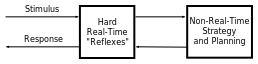
\includegraphics{advsync/rt-reflexes}}
\caption{Real-Time Reflexes}
\label{fig:advsync:Real-Time Reflexes}
\end{figure}

한가지 방법은 많은 링러타임 시스템이 생체 신경 시스템을 닮아서 응답시간은
\cref{fig:advsync:Real-Time Reflexes} 에 그려진 것처럼 리얼타임 반응부터 비
리얼타임 전략화와 계획까지 다양하다는 사실을 인식하는 겁니다.
센서로부터 값을 읽거나 구동기를 제어하는 것 같은 하드 리얼타임 반응은 단일 CPU
나 FPGA 같은 특수 목적 하드웨어에서 실시간으로 동작합니다.
어플리케이셔의 비 리얼타임 전략 짜기나 계획 짜기 부분은 나머지 CPU 에서
수행횝니다.
전략짜기와 계획 짜기는 통계적 분석, 주기적 측정, 사용자 인터페이스, 공급망
활동, 그리고 준비를 포함할 수도 있습니다.
높은 컴퓨팅 부하의 준비 활동을 예로 들어보면,
\pararef{sec:advsync:Real-World Real-Time Specifications}
에서 이야기한 껍질 벗기기 어플리케이션을 다시 생각해 보십시오.
하나의 CPU 가 하나의 통나무를 벗기는데 필요한 높은 속력의 리얼타임 연산을 하는
동안, 나머지 CPU 들은 고품질 나무의 가장 큰 원통을 얻기 위해 다음 통나무를
어떻게 위치시킬지 결정하기 위해 다음 통나무의 크기와 모양을 분석하고 있을 수도
있습니다.
많은 어플리케이션은 비 리얼타임과 리얼타임 컴포넌트를 가지고 있는 것으로
드러났으므로~\cite{RobertBerry2008IBMSysJ}, 이 방법은 전통적 리얼타임 분석이
현대의 멀티코어 하드웨어와 결합되게 하는데 종종 사용될 수 있습니다.

\iffalse

One approach is to recognize the fact that many real-time systems
resemble biological nervous systems, with responses ranging from
real-time reflexes to non-real-time strategizing and planning,
as depicted in
\cref{fig:advsync:Real-Time Reflexes}.
The hard real-time reflexes, which read from sensors and control
actuators, run real-time on a single CPU or on special-purpose hardware
such as an FPGA.
The non-real-time strategy and planning portion of the application runs
on the remaining CPUs.
Strategy and planning activities might include statistical analysis,
periodic calibration, user interface, supply-chain activities, and
preparation.
For an example of high-compute-load preparation activities, think back
to the veneer-peeling application discussed in
\pararef{sec:advsync:Real-World Real-Time Specifications}.
While one CPU is attending to the high-speed real-time computations
required to peel one log, the other CPUs might be analyzing the size
and shape of the next log in order to determine how to position the
next log so as to obtain the largest cylinder of high-quality wood.
It turns out that many applications have non-real-time and real-time
components~\cite{RobertBerry2008IBMSysJ}, so this approach can
often be used to allow traditional real-time analysis to be combined
with modern multicore hardware.

\fi

간단한 방법은 하나의 하드웨어 쓰레드만 남겨둬서 이미 정착된 단일 프로세서
리얼타임 컴퓨팅의 수학으로 되돌아가는 겁니다.
그러나, 이 방법은 잠재적 비용과 전력 효율성 이득을 포기합니다.
그러나, 이 장점을 얻기 위해서는
\cref{chp:Hardware and its Habits} 에서 다룬 병렬 성능 장애들을 극복하는 것이
필요하며 평균만이 아니라 최악의 경우를 대비해야 합니다.

따라서 병렬 리얼타임 시스템을 구현하는 것은 상당히 어려울 수 있습니다.
이를 넘어서기 위한 여러 방법들이 다음 섹션에 소개됩니다.

\iffalse

Another trivial approach is to shut off all but one hardware thread so as
to return to the settled mathematics of uniprocessor real-time
computing.
However, this approach gives up potential cost and energy-efficiency
advantages.
That said, obtaining these advantages requires overcoming the parallel
performance obstacles covered in
\cref{chp:Hardware and its Habits},
and not merely on average, but instead in the worst case.

Implementing parallel real-time systems can therefore be quite a
challenge.
Ways of meeting this challenge are outlined in the following section.

\fi

\subsection{Implementing Parallel Real-Time Systems}
\label{sec:advsync:Implementing Parallel Real-Time Systems}

우리는 두개의 주요 리얼타임 시스템, 즉 event-driven 과 polling 을 살펴볼
겁니다.
Event-driven 리얼타임 시스템은 대부분의 시간을 idle 상태로 지내며 운영체제에
의해 어플리케이션에 전달된 이벤트에 리얼타임으로 반응합니다.
대안적으로, 이 시스템은 비 리얼타임 워크로드를 뒤에서 수행할 수 있습니다.
Polling 리얼타임 시스템은 CPU 에 제한되어 있고 입력을 읽어오고 출력을
업데이트하는 짧은 반복문을 갖는 리얼타임 쓰레드를 가집니다.
이 짧은 polling 반복은 종종 완전히 사용자 모드에서 동작해서 어플리케이션의
user-mode 주소 공간에 매핑된 하드웨어 레지스터를 읽고 쓸 수 있습니다.
대안적으로, 어떤 어플리케이션들은 이 polling 반복을 커널에 위치시키는데 예를
들면 load 할 수 있는 커널 모듈을 사용하는 겁니다.

\iffalse

We will look at two major styles of real-time systems, event-driven and
polling.
An event-driven real-time system remains idle much of the time, responding
in real time to events passed up through the operating system to the
application.
Alternatively, the system could instead be running a background
non-real-time workload.
A polling real-time system features a real-time thread that is CPU
bound, running in a tight loop that polls inputs and updates outputs on
each pass.
This tight polling loop often executes entirely in user mode, reading from
and writing to hardware registers that have been mapped into the user-mode
application's address space.
Alternatively, some applications place the polling loop into the kernel,
for example, using loadable kernel modules.

\fi

\begin{figure}[tb]
\centering
\resizebox{3in}{!}{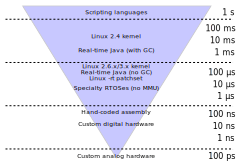
\includegraphics{advsync/rt-regimes}}
\caption{Real-Time Response Regimes}
\label{fig:advsync:Real-Time Response Regimes}
\end{figure}

선택된 스타일과 관계 없이, 리얼타임 시스템을 구현하는데 사용되는 방법은 기한에
종속적일텐데, 예를 들면
\cref{fig:advsync:Real-Time Response Regimes} 에 보인 것과 같습니다.
이 그림의 꼭대기로부터 보면, 여러분이 1초가 넘는 응답시간에도 문제 없다면
여러분의 리얼타임 어플리케이션을 구현하는데 스크립트 언어를 사용할 수도 있을
겁니다---그리고 스크립트 언어는 놀랍도록 자주 사용됩니다만, 제가 이를 꼭
추천해야 할 이유는 아닙니다.
요구되는 응답시간이 수십 밀리세컨드를 넘는다면 오래된 2.4 버전의 리눅스 커널이
사용될 수 있는데, 역시 제가 이를 꼭 추천해야 할 이유는 아닙니다.
특수한 리얼타임 Java 구현은 garbage collector 를 사용하면서도 수 밀리세컨드의
리얼타임 응답시간을 제공할 수 있습니다.
리눅스 2.6.x 와 3.x 커널은 주의 깊게 구성되고 튜닝되고 리얼타임 친화적
하드웨어에서 수행된다면 수백 마이크로세컨드의 리얼타임 응답시간을 제공할 수
있습니다.
특수 리얼타임 Java 구현은 garbage collector 의 사용이 주의 깊게 막아진다면 100
마이크로세컨드 미만의 리얼타임 응답시간을 제공할 수 있습니다.
(하지만 garbage collector 의 사용을 제한함은 Java 의 거대한 표준 라이브러리
사용을 막아서 Java 의 생산성 이득을 막음을 알아두십시오.)
리눅스 4.x 와 5.x 커널은 100 밀리세컨드 미만의 응답시간을 제공합니다만 2.6.x 와
3.x 커널과 같은 주의가 필요합니다.
\rt\ 패치셋을 포함한 리눅스 커널은 20 마이크로세컨드 미만의 응답시간을 제공할
수 있으며, MMU 없이 동작하는 특수 리얼타임 운영체제들은 (RTOS들) 10
마이크로세컨드 미만의 응답시간을 제공할 수 있습니다.
마이크로세컨드 미만 응답시간을 얻는데에는 손으로 짜여진 어셈블리나 심지어 특수
목적 하드웨어가 필요합니다.

\iffalse

Regardless of the style chosen, the approach used to implement a real-time
system will depend on the deadlines, for example, as shown in
\cref{fig:advsync:Real-Time Response Regimes}.
Starting from the top of this figure, if you can live with response times in
excess of one second, you might well be able to use scripting languages
to implement your real-time application---and scripting languages are
in fact used surprisingly often, not that I necessarily recommend this
practice.
If the required latencies exceed several tens of milliseconds,
old 2.4 versions of the Linux kernel can be used, not that I necessarily
recommend this practice, either.
Special real-time Java implementations can provide real-time response
latencies of a few milliseconds, even when the garbage collector is
used.
The Linux 2.6.x and 3.x kernels can provide real-time latencies of
a few hundred microseconds if carefully configured, tuned, and run
on real-time friendly hardware.
Special real-time Java implementations can provide real-time latencies
below 100 microseconds if use of the garbage collector is carefully avoided.
(But note that avoiding the garbage collector means also avoiding
Java's large standard libraries, thus also avoiding Java's productivity
advantages.)
The Linux 4.x and 5.x kernels can provide deep sub-hundred-millisecond
latencies, but with all the same caveats as for the 2.6.x and 3.x kernels.
A Linux kernel incorporating the \rt\ patchset can provide latencies
well below 20 microseconds, and specialty real-time operating systems (RTOSes)
running without MMUs can provide sub-ten-microsecond
latencies.
Achieving sub-microsecond latencies typically requires hand-coded assembly
or even special-purpose hardware.

\fi

물론, 스택 전반에 대한 주의 깊은 구성과 튜닝이 필요합니다.
특히, 하드웨어나 펌웨어가 리얼타임 응답시간을 제공하지 못한다면 소프트웨어가
잃어버린 시간을 위해 할 수 있는 건 없습니다.
더 나쁜 것이, 고성능 하드웨어는 가끔 더 좋은 처리량을 위해 최악의 경우 행동을
희생합니다.
실제로, 인터럽트가 불능화 된 상태에서 도는 짧은 반복문에서의 타이밍은 고품질
난수 생성기의 기본을 제공할 수
있습니다~\cite{PeterOkech2009InherentRandomness}.
더 나아가서, 일부 펌웨어는 다양한 관리 업무를 위해 사이클을 훔치기도 하는데
어떤 경우에는 희생자 CPU 의 하드웨어 클락을 재 프로그래밍 시켜서 그 기록을
지우기까지 합니다.
물론, 사이클 훔치기는 가상화 환경에서는 예상된 행동입니다만 사람들은 가상화
환경에서의 리얼타임 응답을 위해 작업하고
있습니다~\cite{ThomasGleixner2012KVMrealtime,JanKiszka2014virtRT}.
따라서 여러분의 하드웨어와 펌웨어의 리얼타임 기능을 평가하는게 무척 중요합니다.

하지만 좋은 리얼타임 하드웨어와 펌웨어가 있다면 스택의 다음 단계는 운영체제로,
다음 섹션에서 이를 다룹니다.

\iffalse

Of course, careful configuration and tuning are required all the way down
the stack.
In particular, if the hardware or firmware fails to provide real-time
latencies, there is nothing that the software can do to make up for the
lost time.
Worse yet, high-performance hardware sometimes sacrifices worst-case behavior
to obtain greater throughput.
In fact, timings from tight loops run with interrupts disabled can
provide the basis for a high-quality random-number
generator~\cite{PeterOkech2009InherentRandomness}.
Furthermore, some firmware does cycle-stealing to carry out various
housekeeping tasks, in some cases attempting to cover its tracks by
reprogramming the victim CPU's hardware clocks.
Of course, cycle stealing is expected behavior in virtualized
environment, but people are nevertheless working towards real-time
response in virtualized
environments~\cite{ThomasGleixner2012KVMrealtime,JanKiszka2014virtRT}.
It is therefore critically important to evaluate your hardware's and
firmware's real-time capabilities.

But given competent real-time hardware and firmware, the next
layer up the stack is the operating system, which is covered in
the next section.

\fi

\subsection{Implementing Parallel Real-Time Operating Systems}
\label{sec:advsync:Implementing Parallel Real-Time Operating Systems}

\begin{figure}[tb]
\centering
\resizebox{2.2in}{!}{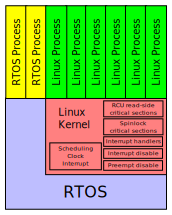
\includegraphics{advsync/Linux-on-RTOS}}
\caption{Linux Ported to RTOS}
\label{fig:advsync:Linux Ported to RTOS}
\end{figure}

리얼타임 시스템을 구현하기 위한 여러 전략이 있습니다.
한가지 방법은 범용 비 리얼타임 OS 를 특수 목적 리얼타임 운영체제 (RTOS) 위에
포팅하는 것으로,
\cref{fig:advsync:Linux Ported to RTOS} 에 보여진 것과 같습니다.
초록색 ``Linux Process'' 박스들은 리눅스 커널에서 돌아가는 비 리얼타임
프로세스를 나타내며, 노란 ``RTOS Process'' 박스들은 RTOS 에서 돌아가는 리얼타임
프로세스들을 나타냅니다.

이는 리눅스 커널이 리얼타임 기능을 얻기 전까지 매우 대중적인 전략이었으며,
여전히 사용됩니다~\cite{Xenomai2014,VictorYodaiken2004a}.
그러나, 이 방법은 어플리케이션이 RTOS 에서 돌아가는 부분과 리눅스에서 돌아가는
부분으로 분리될 것을 필요로 합니다.
예를 들어 RTOS 로부터의 POSIX 시스템콜을 리눅스에서 도는 관리 쓰레드로 넘기는
것과 같이 두 환경을 비슷해 보이게 하는 것은 가능하나, 언제나 깔끔하게 떨어지지
않는 부분이 있습니다.

\iffalse

There are a number of strategies that may be used to implement a
real-time system.
One approach is to port a general-purpose non-real-time OS on top
of a special purpose real-time operating system (RTOS), as shown in
\cref{fig:advsync:Linux Ported to RTOS}.
The green ``Linux Process'' boxes represent non-real-time processes
running on the Linux kernel, while the yellow ``RTOS Process''
boxes represent real-time processes running on the RTOS\@.

This was a very popular approach before the Linux kernel gained
real-time capabilities, and is still in
use~\cite{Xenomai2014,VictorYodaiken2004a}.
However, this approach requires that the application be split into
one portion that runs on the RTOS and another that runs on Linux.
Although it is possible to make the two environments look similar,
for example, by forwarding POSIX system calls from the RTOS to a
utility thread running on Linux, there are invariably rough edges.

\fi

또한, RTOS 는 하드웨어와 리눅스 커널 둘 다와 상호작용해야 해서, 하드웨어와 커널
양쪽에의 변경에 대한 상당한 관리를 요합니다.
더 나아가, 그런 RTOS 각각은 종종 자신만의 시스템콜 인터페이스와 시스템
라이브러리 집합을 가져서, 에코시스템과 개발자들을 분열시킬 수 있습니다.
실제로, 이 문제들은 RTOS 와 리눅스의 결합을 이끈 것으로 보여지는데, 이 방법은
RTOS 의 완전한 리얼타임 능력에의 접근을 허용하는 한편 어플리케이션의 비
리얼타임 코드는 리눅스의 오픈소스 에코시스템에 완전한 접근을 허용했기
때문입니다.

\iffalse

In addition, the RTOS must interface to both the hardware and to
the Linux kernel, thus requiring significant maintenance with
changes in both hardware and kernel.
Furthermore, each such RTOS often has its own system-call interface
and set of system libraries, which can balkanize both ecosystems and
developers.
In fact, these problems seem to be what drove the combination of
RTOSes with Linux, as this approach allowed access to the full real-time
capabilities of the RTOS, while allowing the application's non-real-time
code full access to Linux's open-source ecosystem.

\fi

\begin{figure*}[p]
\centering
\resizebox{4.4in}{!}{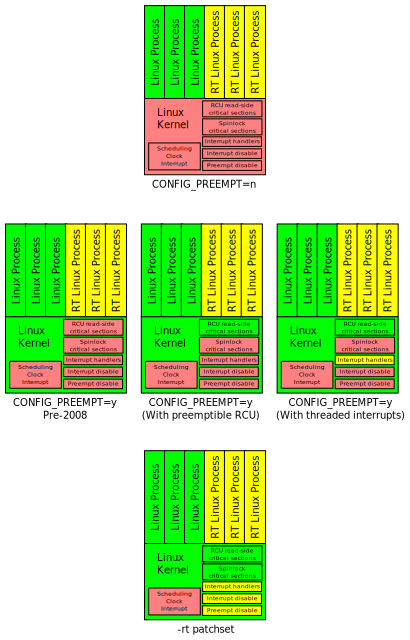
\includegraphics{advsync/preemption}}
\caption{Linux-Kernel Real-Time Implementations}
\label{fig:advsync:Linux-Kernel Real-Time Implementations}
\end{figure*}

RTOS 와 리눅스 커널을 결합시키는 건 리눅스 커널이 최소한의 리얼타임 기능만을
가지고 있던 때에는 영리하고 유용한 단기적 방법이었습니다만, 이는 또한 리눅스
커널에 리얼타임 기능을 추가하는 동기가 되었습니다.
이 목표를 향한 진행이
\cref{fig:advsync:Linux-Kernel Real-Time Implementations} 에 보여 있습니다.
윗열은 preemption 이 불능화된, 따라서 리얼타임 기능을 갖지 못한 리눅스 커널을
보입니다.
가운데 열은 preemption 이 허용된 상태에서의 메인라인 리눅스 커널의 리얼타임
기능이 늘어나는 과정을 보입니다.
마지막으로, 아랫열은 \rt\ 패치셋이 적용되어 리얼타임 기능이 최대화 된 상태의
리눅스 커널을 보입니다.
\rt\ 패치셋으로부터의 기능이 메인라인에 더해졌으므로, 메인라인 리눅스 커널의
기능은 시간에 따라 점차 늘어가고 있습니다.
그러나, 가장 필요한 리얼타임 어플리케이션은 \rt\ 패치셋을 계속 사용하고
있습니다.

\iffalse

Although pairing RTOSes with the Linux kernel was a clever and useful
short-term response during the time that the Linux kernel had minimal
real-time capabilities, it also motivated adding real-time capabilities
to the Linux kernel.
Progress towards this goal is shown in
\cref{fig:advsync:Linux-Kernel Real-Time Implementations}.
The upper row shows a diagram of the Linux kernel with preemption disabled,
thus having essentially no real-time capabilities.
The middle row shows a set of diagrams showing the increasing real-time
capabilities of the mainline Linux kernel with preemption enabled.
Finally, the bottom row shows a diagram of the Linux kernel with the
\rt\ patchset applied, maximizing real-time capabilities.
Functionality from the \rt\ patchset is added to mainline,
hence the increasing capabilities of the mainline Linux kernel over time.
Nevertheless, the most demanding real-time applications continue to use
the \rt\ patchset.

\fi

\cref{fig:advsync:Linux-Kernel Real-Time Implementations}
의 꼭대기에 보인 preemption 불가 커널은 \co{CONFIG_PREEMPT=n} 과 함께
빌드외어서 리눅스 커널 내에서의 수행은 preemption 될 수 없습니다.
이는 커널의 리얼타임 응답시간은 리눅스 커널의 가장 긴, 실제로도 긴, 코드 경로에
제한됨을 의미합니다.
그러나, 사용자 모드 수행은 preemption 가능하므로 우상단에 보인 리얼타임 리눅스
프로세스들은 좌상단에 보인 비 리얼타임 리눅스 프로세스를 비 리얼타임 리눅스
프로세스가 사용자 모드에서 수행중인 동안에는 언제든 preempt 시킬 수 있을
겁니다.

\iffalse

The non-preemptible kernel shown at the top of
\cref{fig:advsync:Linux-Kernel Real-Time Implementations}
is built with \co{CONFIG_PREEMPT=n}, so that execution within the Linux
kernel cannot be preempted.
This means that the kernel's real-time response latency is bounded below
by the longest code path in the Linux kernel, which is indeed long.
However, user-mode execution is preemptible, so that one of the
real-time Linux processes shown in the upper right may preempt any of the
non-real-time Linux processes shown in the upper left anytime the
non-real-time process is executing in user mode.

\fi

\cref{fig:advsync:Linux-Kernel Real-Time Implementations}
의 가운데 열은 리눅스의 preemption 가능한 커널 개발 과정의 세 단계 (왼쪽에서
오른쪽으로) 를 보입니다.
세 단계 모두에서, 리눅스 커널의 대부분의 프로세스 단계 코드는 preeemption 될 수
있습니다.
이는 물론 리얼타임 응답시간을 크게 개선합니다만 여전히 RCU read-side 크리티컬
섹션, spinlock 크리티컬 섹션, 인터럽트 핸들러, 인터럽트가 불능화된 코드 구역,
그리고 preemption 이 불능화된 코드 구역에서는 이 그림의 가운데 열의 가장 왼쪽의
빨간 박스들로 보인 것처럼 여전히 preemption 이 불가능합니다.
Preemption 가능한 RCU 의 발전은 가장 오른쪽 다이어그램이 보이듯 RCU read-side
크리티컬 섹션이 preemption 가능하게 만들었습니다.
물론, 다른 리얼타임 기능이 시간의 흐름에 따라 더해졌습니다만, 이 모두를 이
다이어그램에 쉽게 보일 수가 없습니다.
그에 대해서는
\cref{sec:advsync:Event-Driven Real-Time Support} 에서 이야기 하겠습니다.

\iffalse

The middle row of
\cref{fig:advsync:Linux-Kernel Real-Time Implementations}
shows three stages (from left to right) in the development of Linux's
preemptible kernels.
In all three stages, most process-level code within the Linux kernel
can be preempted.
This of course greatly improves real-time response latency, but
preemption is still disabled
within RCU read-side critical sections,
spinlock critical sections,
interrupt handlers,
interrupt-disabled code regions, and
preempt-disabled code regions, as indicated by the red boxes in the
left-most diagram in the middle row of the figure.
The advent of preemptible RCU allowed RCU read-side critical sections
to be preempted, as shown in the central diagram,
and the advent of threaded interrupt handlers allowed device-interrupt
handlers to be preempted, as shown in the right-most diagram.
Of course, a great deal of other real-time functionality was added
during this time, however, it cannot be as easily represented on this
diagram.
It will instead be discussed in
\cref{sec:advsync:Event-Driven Real-Time Support}.

\fi

\cref{fig:advsync:Linux-Kernel Real-Time Implementations}
의 아랫열은 쓰레드화된 (그리고 따라서 preemption 가능한) 많은 기기를 위한
인터럽트 핸들러를 갖는, 따라서 이 드라이버들의 ``인터럽트 불능화된'' 영역들을
preemption 가능하게 하는 \rt\ 패치셋을 보입니다.
이 드라이버들은 각 드라이버의 프로세스 단계 부분들을 쓰레드화된 인터럽트
핸들러와 동기화 시키기 위해 락킹을 대신 사용합니다.
마지막으로, 어떤 경우에는 preemption 의 불능화가 migration 불능화로 대체됩니다.
이는 \rt\ 패치셋을 사용해 수행되는 많은 시스템에서의 상당한 응답시간 개선을
보입니다~\cite{Reghenzani:2019:RLK:3309872.3297714,DanielBristot2019RTtrace}.

\iffalse

The bottom row of
\cref{fig:advsync:Linux-Kernel Real-Time Implementations}
shows the \rt\ patchset, which features threaded (and thus preemptible)
interrupt handlers for many devices, which also allows the corresponding
``interrupt-disabled'' regions of these drivers to be preempted.
These drivers instead use locking to coordinate the process-level
portions of each driver with its threaded interrupt handlers.
Finally, in some cases, disabling of preemption is replaced by
disabling of migration.
These measures result in excellent response times in many systems running
the \rt\ patchset~\cite{Reghenzani:2019:RLK:3309872.3297714,DanielBristot2019RTtrace}.

\fi

\begin{figure}[tb]
\centering
\resizebox{2.5in}{!}{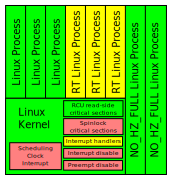
\includegraphics{advsync/nohzfull}}
\caption{CPU Isolation}
\label{fig:advsync:CPU Isolation}
\end{figure}

마지막 방법은 리얼타임 프로세스를 방해할 수 있는 모든 것을 치우는 것으로,
\cref{fig:advsync:CPU Isolation} 에 보인 것처럼 이 프로세스가 필요한 모든 CPU
로부터 다른 일들을 모두 제거해 버리는 겁니다.
이는 3.10 리눅스 커널에서 \co{CONFIG_NO_HZ_FULL} Kconfig 패러미터를 통해
구현되었습니다~\cite{JonCorbet2013NO-HZ-FULL,FredericWeisbecker2013nohz}.
이 방법은 최소 하나의 \emph{관리 CPU}, 예를 들면 커널 daemon 같은 것이 뒤에서
수행되게 할 것을 필요로 함을 알아두는게 중요합니다.
그러나, 비 관리 CPU 에서 수행될 수 있는 태스크가 단 하나일 때에는 스케쥴링 클락
인터럽트가 해당 CPU 에서는 꺼져버려서 상관과 \emph{OS jitter} 의 중요한 원천이
제거됩니다.
일부 예외와 함께, 이 커널은 다른 일들이 비 관리 CPU 로부터 사라지게 하지는
않으나 특정 CPU 에 하나의 태스크만 수행 가능할 때의 성능을 낫게 만들어 줍니다.
여러 userspace 도구들이 특정 CPU 가 두개 이상의 수행 가능 태스크를 갖지 못하게
만드는데 사용될 수 있습니다.
올바르게 구성된다면, \co{CONFIG_NO_HZ_FULL} 은 베어메탈 시스템의 그것에
근접하는 리얼타임 쓰레드 수준의 성능을
제공합니다~\cite{AbdullahAljuhni2018nohzfull}.

\iffalse

A final approach is simply to get everything out of the way of the
real-time process, clearing all other processing off of any CPUs that
this process needs, as shown in \cref{fig:advsync:CPU Isolation}.
This was implemented in the 3.10 Linux kernel via the \co{CONFIG_NO_HZ_FULL}
Kconfig parameter~\cite{JonCorbet2013NO-HZ-FULL,FredericWeisbecker2013nohz}.
It is important to note that this approach requires at least one
\emph{housekeeping CPU} to do background processing, for example running
kernel daemons.
However, when there is only one runnable task on a given non-housekeeping CPU,
scheduling-clock interrupts are shut off on that CPU, removing an important
source of interference and \emph{OS jitter}.
With a few exceptions, the kernel does not force other processing off of the
non-housekeeping CPUs, but instead simply provides better performance
when only one runnable task is present on a given CPU\@.
Any number of userspace tools may be used to force a given CPU to have
no more that one runnable task.
If configured properly, a non-trivial undertaking, \co{CONFIG_NO_HZ_FULL}
offers real-time threads levels of performance that come close to those of
bare-metal systems~\cite{AbdullahAljuhni2018nohzfull}.

\fi

물론, 이 방법들 가운데 무엇이 리얼타임 시스템을 위한 최고의 방법인지에 대해선
상당한 논쟁이 있었으며 그 논쟁은 상당한 시간동안
진행되었습니다~\cite{JonCorbet2004RealTimeLinuxPart1,JonCorbet2004RealTimeLinuxPart2}.
보통 그렇듯, 답은 ``경우에 따라 다르다'' 인 듯 보이는데, 다음 섹션들에서 이를
다룹니다.
\Cref{sec:advsync:Event-Driven Real-Time Support}
는 이벤트 주도 리얼타임 시스템을 다루고,
\Cref{sec:advsync:Polling-Loop Real-Time Support}
는 CPU-제한 polling 반복문을 사용하는 리얼타임 시스템을 알아봅니다.

\iffalse

There has of course been much debate over which of these approaches
is best for real-time systems, and this debate has been going on for
quite some
time~\cite{JonCorbet2004RealTimeLinuxPart1,JonCorbet2004RealTimeLinuxPart2}.
As usual, the answer seems to be ``It depends,'' as discussed in the
following sections.
\Cref{sec:advsync:Event-Driven Real-Time Support}
considers event-driven real-time systems, and
\Cref{sec:advsync:Polling-Loop Real-Time Support}
considers real-time systems that use a CPU-bound polling loop.

\fi

\subsubsection{Event-Driven Real-Time Support}
\label{sec:advsync:Event-Driven Real-Time Support}

이벤트 주도 리얼타임 어플리케이션을 위한 운영체제 지원은 상당히 많은 게 필요할
수 있습니다만 이 섹션은 그 중 몇가지, 즉 타이머, 쓰레드 인터럽트, 우선순위
계승, preemptible RCU, 그리고 preemptible spinlock 에만 집중합니다.

\iffalse

The operating-system support required for event-driven real-time
applications is quite extensive, however, this section will focus
on only a few items, namely
timers,
threaded interrupts,
priority inheritance,
preemptible RCU,
and
preemptible spinlocks.

\fi

\paragraph{Timer} 는 리얼타임 오퍼레이션들을 위해 분명 무척 중요합니다.
어쨌건, 무언가가 특정 시간에 완료되었다고 기술할 수가 없다면, 그 시간에 어떻게
응답을 하겠습니까?
비 리얼타임 시스템에서조차도, 많은 수의 타이머가 만들어졌으며, 따라서 그것들은
아주 효율적으로 다루어져야 합니다.
예로는 TCP 연결을 위한 재전송 타이머 (거의 항상 만료 전에 취소될),\footnote{
	최소한 합리적으로 낮은 패킷 손실율을 가정하면요!}
시간이 명시된 지연 (드물게 취소될, \co{sleep(1)} 과 같은), 그리고 \co{poll()}
시스템콜을 위한 시간 기반 종료 (거의 항상 만료 전에 취소될) 등이 있겠습니다.
따라서 그런 타이머를 위한 좋은 데이터 구조는 추가와 제거 기능이 빠르고 추가된
타이머의 갯수에 대해 $\O{1}$ 인 우선순위 queue 가 될 겁니다.

이 목적을 위한 고전적인 데이터 구조는 \emph{calendar queue} 로, 리눅스
커널에서는 \co{timer wheel} 이라 불립니다.
이 오래된 데이터 구조는 이산적 이벤트 시뮬레이션에도 널리 사용됩니다.
아이디어는 시간은 수치화 된다는 것으로, 예를 들어 리눅스 커널에서 시간 단위는
스케쥴링 클락 인터럽트 기간입니다.
시간은 정수로 표현될 수 있으며, 정수가 아닌 시간을 위한 타이머를 추가하려는
시도는 가까운 정수 시간 단위로 변환될 겁니다.

\iffalse

\paragraph{Timers} are clearly critically important for real-time
operations.
After all, if you cannot specify that something be done at a specific
time, how are you going to respond by that time?
Even in non-real-time systems, large numbers of timers are generated,
so they must be handled extremely efficiently.
Example uses include retransmit timers for TCP connections (which are
almost always canceled before they have a chance to fire),\footnote{
	At least assuming reasonably low packet-loss rates!}
timed delays (as in \co{sleep(1)}, which are rarely canceled),
and timeouts for the \co{poll()} system call (which are often
canceled before they have a chance to fire).
A good data structure for such timers would therefore be a priority queue
whose addition and deletion primitives were fast and $\O{1}$ in the number
of timers posted.

The classic data structure for this purpose is the \emph{calendar queue},
which in the Linux kernel is called the \co{timer wheel}.
This age-old data structure is also heavily used in discrete-event
simulation.
The idea is that time is quantized, for example, in the Linux kernel,
the duration of the time quantum is the period of the scheduling-clock
interrupt.
A given time can be represented by an integer, and any attempt to post
a timer at some non-integral time will be rounded to a convenient nearby
integral time quantum.

\fi

한가지 단순한 구현은 시간의 아래쪽 비트들로 인덱스 되는 배열을 할당하는 것일
겁니다.
이는 이론상으로는 동작합니다만, 실제 시스템에서는 거의 항상 취소되는 긴 시간의
타임아웃을 (예를 들어, TCP session 을 위한 두시간짜리 keepalive 타임아웃) 무척
많이 생성합니다.
이 긴 시간의 타임아웃은 작은 배열에서 문제를 일으킬 수 있는데, 대부분의 시간은
아직 만료되지 않은 타임아웃을 넘기느라 낭비될 것이기 때문입니다.
다른 한편, 우아하게 많은 수의 장기간 타임아웃을 수용할 수 있는 충분히 큰 배열은
너무 많은 메모리를 소모할텐데, 특히 성능과 확장성에 대한 염려는 각 CPU 마다
그런 배열을 하나씩 요구할 것이라는 점에서 그렇습니다.

\iffalse

One straightforward implementation would be to allocate a single array,
indexed by the low-order bits of the time.
This works in theory, but in practice systems create large numbers of
long-duration timeouts (for example, the two-hour keepalive timeouts for TCP
sessions) that are almost always canceled.
These long-duration timeouts cause problems for small arrays because
much time is wasted skipping timeouts that have not yet expired.
On the other hand, an array that is large enough to gracefully accommodate
a large number of long-duration timeouts would consume too much memory,
especially given that performance and scalability concerns require one
such array for each and every CPU\@.

\fi

\begin{figure}[tb]
\centering
\resizebox{2.0in}{!}{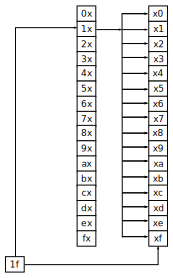
\includegraphics{advsync/timerwheel}}
\caption{Timer Wheel}
\label{fig:advsync:Timer Wheel}
\end{figure}

이 문제를 해결하는 일반적인 방법은 계층적인 여러 배열을 제공하는 겁니다.
이 계층의 가장 아랫단에서 각 배열 원소는 하나의 시간 단위를 의미합니다.
두번째 계층에서, 각 배열 원소는 $N$ 개의 시간 유닛을 의미하는데 $N$ 은 각
배열의 원소 수입니다.
세번째 계층에서, 각 배열 원소는 $N^2$ 시간 유닛을 의미하며, 그렇게 계층의
위쪽으로 반복됩니다.
이 방법은 개별적 배열들이 다른 비트를 통해 인덱스 될 수 있게 하는데,
\cref{fig:advsync:Timer Wheel} 에서 비현실적으로 작은 8 비트 클락을 보인 것과
같습니다.
여기서, 각 원소는 16 개의 원소를 가지므로, 시간의 아랫쪽 네개의 비트는 (현재
\co{0xf}) 아랫단 (오른쪽) 배열을 인덱스 하며, 다음 네개의 비트 (현재 \co{0x1})
은 그 윗 단계를 인덱스 합니다.
따라서, 우린 16 개의 원소를 갖는 두개의 배열을 가져서 총 32개 원소를 갖는데,
이는 하나의 배열을 사용했다면 필요했을 256개 원소 배열보다 훨씬 작습니다.

이 방법은 처리량 기반 시스템에서 무척 잘 동작합니다.
각 타이머 오퍼레이션은 작은 상수의 $\O{1}$ 이며, 각 타이머 원소는 최대 $m+1$ 회
접근되는데, $m$ 은 계층의 전체 높이입니다.

\iffalse

A common approach for resolving this conflict is to provide multiple
arrays in a hierarchy.
At the lowest level of this hierarchy, each array element represents
one unit of time.
At the second level, each array element represents $N$ units of time,
where $N$ is the number of elements in each array.
At the third level, each array element represents $N^2$ units of time,
and so on up the hierarchy.
This approach allows the individual arrays to be indexed by different
bits, as illustrated by
\cref{fig:advsync:Timer Wheel}
for an unrealistically small eight-bit clock.
Here, each array has 16 elements, so the low-order four bits of the time
(currently \co{0xf}) index the low-order (rightmost) array, and the
next four bits (currently \co{0x1}) index the next level up.
Thus, we have two arrays each with 16 elements, for a total of 32 elements,
which, taken together, is much smaller than the 256-element array that
would be required for a single array.

This approach works extremely well for throughput-based systems.
Each timer operation is $\O{1}$ with small constant, and each timer
element is touched at most $m+1$ times, where $m$ is the number of
levels.

\fi

\begin{figure}[tb]
\centering
\resizebox{3.0in}{!}{\includegraphics{cartoons/1kHz}}
\caption{Timer Wheel at 1\,kHz}
\ContributedBy{Figure}{fig:advsync:Timer Wheel at 1kHz}{Melissa Broussard}
\end{figure}

\begin{figure}[tb]
\centering
\resizebox{3.0in}{!}{\includegraphics{cartoons/100kHz}}
\caption{Timer Wheel at 100\,kHz}
\ContributedBy{Figure}{fig:advsync:Timer Wheel at 100kHz}{Melissa Broussard}
\end{figure}

불행히도, timer wheel 은 리얼타임 시스템에서 두가지 이유로 잘 동작하지
못합니다.
첫번째 이유는
\cref{fig:advsync:Timer Wheel at 1kHz,fig:advsync:Timer Wheel at 100kHz}
에 보여진 것처럼 타이머 정확도와 오버헤드 사이의 거친 트레이드오프가 있다는
겁니다.
\Cref{fig:advsync:Timer Wheel at 1kHz} 에서, 타이머 처리는 밀리세컨드당 한번만
발생하여, 많은 (그러나 전부는 아닌!) 워크로드에 있어서 받아들여지기 충분히 낮은
오버헤드를 유지합니다만, 이는 또한 밀리세컨드 단위보다 작은 단위의 타임아웃은
불가능함을 의미합니다.
다른 한편, \cref{fig:advsync:Timer Wheel at 100kHz} 는 10 마이크로세컨드마다
타이머 처리가 발생하는 경우를 보이는데, 대부분의 (그러나 전부는 아닌!)
워크로드에게 받아들여지기 충분한 세밀한 시간 단위를 제공하지만, 타이머를 매우
빈번하게 처리하기에 시스템은 다른 일을 할 시간을 충분히 갖지 못할 수도
있습니다.

\iffalse

Unfortunately, timer wheels do not work well for real-time systems, and for
two reasons.
The first reason is that there is a harsh tradeoff between timer
accuracy and timer overhead, which is fancifully illustrated by
\cref{fig:advsync:Timer Wheel at 1kHz,fig:advsync:Timer Wheel at 100kHz}.
In \cref{fig:advsync:Timer Wheel at 1kHz},
timer processing happens only once per millisecond, which keeps overhead
acceptably low for many (but not all!) workloads, but which also means
that timeouts cannot be set for finer than one-millisecond granularities.
On the other hand, \cref{fig:advsync:Timer Wheel at 100kHz}
shows timer processing taking place every ten microseconds, which
provides acceptably fine timer granularity for most (but not all!)
workloads, but which processes timers so frequently that the system
might well not have time to do anything else.

\fi

두번째 이유는 타이머를 높은 단계에서 낮은 단계로 연결되어야 한다는 필요입니다.
\Cref{fig:advsync:Timer Wheel} 로 돌아가서, 우린 윗단 (왼쪽) 배열의 원소에
enqueue 된 모든 타이머는 아랫단 (오른쪽) 배열로 연결되어서 그것들의 시간이
도착했을 때 호출될 수 있게 해야 합니다.
불행히도, 연결을 기다리는 많은 수의 타임아웃이 있을 수 있는데, 큰 수의 단계를
갖는 timer wheel 에서는 특히 그렇습니다.
통계의 힘이 이 연결을 처리량 기반 시스템에서는 문제가 아니게 만듭니다만,
리얼타임 시스템에서는 응답 시간 악화로 문제를 초래할 수 있습니다.

\iffalse

The second reason is the need to cascade timers from higher levels to
lower levels.
Referring back to \cref{fig:advsync:Timer Wheel},
we can see that any timers enqueued on element \co{1x} in the upper
(leftmost) array must be cascaded down to the lower (rightmost)
array so that may be invoked when their time arrives.
Unfortunately, there could be a large number of timeouts
waiting to be cascaded, especially for timer wheels with larger numbers
of levels.
The power of statistics causes this cascading to be a non-problem for
throughput-oriented systems, but cascading can result in problematic
degradations of latency in real-time systems.

\fi

\IfTwoColumn{
\begin{figure*}[tb]
\centering
\resizebox{1.4\twocolumnwidth}{!}{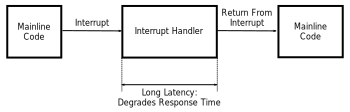
\includegraphics{advsync/irq}}
\caption{Non-Threaded Interrupt Handler}
\label{fig:advsync:Non-Threaded Interrupt Handler}
\end{figure*}
}{}

\IfTwoColumn{
\begin{figure*}[tb]
\centering
\resizebox{1.4\twocolumnwidth}{!}{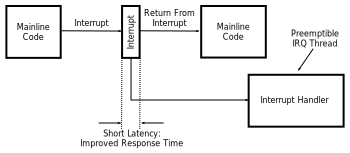
\includegraphics{advsync/threaded-irq}}
\caption{Threaded Interrupt Handler}
\label{fig:advsync:Threaded Interrupt Handler}
\end{figure*}
}{}

물론, 리얼타임 시스템은 단순히 다른 데이터 구조를 사용할 수도 있는데, 예를 들면
heap 이나 tree 같은 것으로, 추가와 삭제 오퍼레이션에서 $\O{1}$ 제한을 포기하고
데이터 구조 유지 오퍼레이션들에서 $\O{\log n}$ 제한을 얻는 겁니다.
이는 특수 목적 RTOS 들에서는 좋은 선택일 수 있으나, 리눅스와 같이 극단적으로
많은 수의 타이머를 지원하는 범용 시스템에서는 비효율적입니다.

리눅스 커널의 \rt\ 패치셋에서 선택한 해결책은 나중의 행동을 스케쥴 하는
타이머와 TCP 패킷 손실과 같은 낮은 가능성의 에러의 처리를 스케쥴 하는
타임아웃을 다르게 처리하는 겁니다.
한가지 핵심 발견은 에러 처리는 일반적으로 특별히 시간에 치명적이지 않으며,
따라서 timer wheel 의 밀리세컨드 단위가 충분히 좋다는 겁니다.
또다른 핵심 발견은 에러 처리 타임아웃은 일반적으로 매우 일찍, 종종 윗단에서
아랫단으로 연결되기 전에 취소된다는 겁니다.
또한, 타이머 이벤트보다 많은 에러 처리 타임아웃을 갖는 시스템이 흔해서 $\O{\log
n}$ 데이터 구조는 타이머 이벤트를 위한 받아들여질 수 있는 수준의 성능을
제공합니다.

\iffalse

Of course, real-time systems could simply choose a different data
structure, for example, some form of heap or tree, giving up
$\O{1}$ bounds on insertion and deletion operations to gain $\O{\log n}$
limits on data-structure-maintenance operations.
This can be a good choice for special-purpose RTOSes, but is inefficient
for general-purpose systems such as Linux, which routinely support
extremely large numbers of timers.

The solution chosen for the Linux kernel's \rt\ patchset is to differentiate
between timers that schedule later activity and timeouts that schedule
error handling for low-probability errors such as TCP packet losses.
One key observation is that error handling is normally not particularly
time-critical, so that a timer wheel's millisecond-level granularity
is good and sufficient.
Another key observation is that error-handling timeouts are normally
canceled very early, often before they can be cascaded.
In addition, systems commonly have many more error-handling timeouts
than they do timer events, so that an $\O{\log n}$ data structure should
provide acceptable performance for timer events.

\fi

그러나, 더 잘할 수도 있는데, 타이머를 연결하는 걸 그냥 거부하는 겁니다.
연결 대신, calendar queue 의 아랫단으로 연결되었어야 할 타이머는 그대로
있습니다.
이는 이 시간 기간 내에서의 몇퍼센트의 에러를 초래합니다만 이게 문제일 수 있는
소수의 상황에서는 tree 기반의 고해상도 타이머 (hrtimers) 를 사용할 수 있습니다.

요약해서, 리눅스 커널의 \rt\ 패치셋은 에러 처리 타임아웃을 위해서는 timer wheel
을 쓰고 타이머 이벤트를 위해선 tree 를 사용해서 각 카테고리에 필요한 품질의
서비스를 제공합니다.

\iffalse

However, it is possible to do better, namely by simply refusing to
cascade timers.
Instead of cascading, the timers that would otherwise have been cascaded
all the way down the calendar queue are handled in place.
This does result in up to a few percent error for the time duration,
but the few situations where this is a problem can instead use tree-based
high-resolution timers (hrtimers).

In short, the Linux kernel's \rt\ patchset uses timer wheels for
error-handling timeouts and a tree for timer events, providing each
category the required quality of service.

\fi

\IfTwoColumn{}{
\begin{figure}[tb]
\centering
\resizebox{1.4\twocolumnwidth}{!}{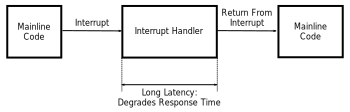
\includegraphics{advsync/irq}}
\caption{Non-Threaded Interrupt Handler}
\label{fig:advsync:Non-Threaded Interrupt Handler}
\end{figure}
}

\paragraph{Threaded interrupts}
는 리얼타임 응답 악화의 심각한 원천, 즉
\cref{fig:advsync:Non-Threaded Interrupt Handler} 에 보인 것과 같은 오래
수행되는 인터럽트 핸들러를 처리하기 위해 사용됩니다.
이 응답시간은 하나의 인터럽트로 큰 수의 이벤트를 전달할 수 있는, 즉 인터럽트
핸들러가 이 이벤트 전체를 처리하기 위해 연장된 시간동안 수행될 것을 의미하는
기기에서 특히 문제가 될 수 있습니다.
더 나빠질 수 있는건 여전히 수행중인 인터럽트 핸들러에게 새 이벤트를 전달할 수
있는 기기들로, 그런 인터럽트 핸들러는 무한히 수행될 수도 있어서 리얼타임 응답을
무한히 악화시킬 수 있습니다.

\iffalse

\paragraph{Threaded interrupts}
are used to address a significant source of degraded real-time latencies,
namely long-running interrupt handlers,
as shown in \cref{fig:advsync:Non-Threaded Interrupt Handler}.
These latencies can be especially problematic for devices that can
deliver a large number of events with a single interrupt, which means
that the interrupt handler will run for an extended period of time
processing all of these events.
Worse yet are devices that can deliver new events to a still-running
interrupt handler, as such an interrupt handler might well run
indefinitely, thus indefinitely degrading real-time latencies.

\fi

\IfTwoColumn{}{
\begin{figure}[tb]
\centering
\resizebox{1.4\twocolumnwidth}{!}{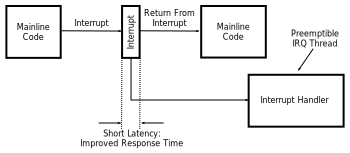
\includegraphics{advsync/threaded-irq}}
\caption{Threaded Interrupt Handler}
\label{fig:advsync:Threaded Interrupt Handler}
\end{figure}
}

이 문제를 해결하는 한가지 방법은 \cref{fig:advsync:Threaded Interrupt Handler}
에 보인 쓰레드화된 인터럽트 (threaded interrupts) 를 사용하는 겁니다.
설정 가능한 우선순위로 수행되며 ㅔreemption 가능한 \IRQ\ 쓰레드의 컨텍스트에서
수행되는 인터럽트 핸들러입니다.
그럼 이 기기 입터럽트 핸들러는 짧은 시간동안만 수행되는데, \IRQ\ 쓰레드가 새
이벤트를 알아차릴 수 있을 만큼만 긴 정도입니다.
그림에서 보였듯, 쓰레드화된 인터럽트는 링러타임 응답을 크게 개선할 수 있는데,
부분적으로는 \IRQ\ 쓰레드의 컨텍스트에서 수행되는 인터럽트 핸들러가 높은
우선순위 리얼타임 쓰레드에게 preemption 당할 수 있기 때문입니다.

\iffalse

One way of addressing this problem is the use of threaded interrupts shown in
\cref{fig:advsync:Threaded Interrupt Handler}.
Interrupt handlers run in the context of a preemptible \IRQ\ thread,
which runs at a configurable priority.
The device interrupt handler then runs for only a short time, just
long enough to make the \IRQ\ thread aware of the new event.
As shown in the figure, threaded interrupts can greatly improve
real-time latencies, in part because interrupt handlers running in
the context of the \IRQ\ thread may be preempted by high-priority real-time
threads.

\fi

하지만 공짜 점심은 없으며 쓰레드화된 인터럽트에게도 단점이 있습니다.
그런 단점 중 하나는 증가되는 인터럽트 응답시간입니다.
인터럽트는 즉각 수행되는 대신, 이 핸들러의 수행 부분은 \IRQ\ 쓰레드가 수행될 수
있을 때까지 미뤄집니다.
물론, 인터럽트를 생성하는 기기가 리얼타임 어플리케이션의 중요 경로에 있지
않다면 이는 문제가 되지 않습니다.

또다른 단점은 잘못 짜여진 높은 우선순위 리얼타임 코드가 인터럽트 핸들러를 기아
상태에 빠지게 할 수 있다는 것으로, 예를 들어 네트워크 코드가 수행되지 못하게
해서 결국 문제를 디버깅 하기 어렵게 만드는 겁니다.
따라서 개발자들은 높은 우선순위 리얼타임 코드를 작성할 때 큰 주의를 기울여야
합니다.
이를 \emph{스파이더맨 원칙} 이라고 부릅니다: 큰 힘에는 큰 책임이 따릅니다.

\iffalse

However, there is no such thing as a free lunch, and there are downsides
to threaded interrupts.
One downside is increased interrupt latency.
Instead of immediately running the interrupt handler, the handler's execution
is deferred until the \IRQ\ thread gets around to running it.
Of course, this is not a problem unless the device generating the interrupt
is on the real-time application's critical path.

Another downside is that poorly written high-priority real-time code
might starve the interrupt handler, for example, preventing networking
code from running, in turn making it very difficult to debug the problem.
Developers must therefore take great care when writing high-priority
real-time code.
This has been dubbed the \emph{Spiderman principle}: With great power
comes great responsibility.

\fi

\paragraph{Priority inheritance} 는 다른것들 가운데에서도 preemption 가능한
인터럽트 핸들러에서 획득되는 락들로 인해 일어날 수
있는 우선순위 역전을~\cite{LuiSha1990PriorityInheritance} 처리하기 위해
사용됩니다.
낮은 우선순위 쓰레드가 락을 잡았는데 중간 우선순위의 쓰레드당 최소 하나는 되는
쓰레드들에 의해 preemption 당한다고 생각해 봅시다.
인터럽트가 발생하면 높은 우선순위 \IRQ\ 쓰레드가 이 중간 우선순위 쓰레드들
가운데 하나를 preempt 하지만 낮은 우선순위 쓰레드가 쥐고 있는 락을 획득하려
히기 전까지만입니다.
불행히도, 이 낮은 우선순위 쓰레드는 수행을 시작하기 전까지 이 락을 높을 수
없는데, 중간 우선순위 쓰레드가 그걸 못하게 하고 있습니다.
따라서 높은 우선순위 \IRQ\ 쓰레드는 중간 우선순위 쓰레드들 중 하나가 CPU 를
놓기 전까지 이 락을 획득하지 못합니다.
요약하자면, 중간 우선순위 쓰레드가 간접적으로 높은 우선순위 \IRQ\ 쓰레드를 막고
있게 되어, 고전적인 우선순위 역전이 형성됩니다.

이 우선순위 역전은 낮은 우선순위 쓰레드는 락을 잡고 있는 동안 인터럽트를 불능화
시켜야 할 것이어서 중간 우선순위 쓰레드가 preempt 시키는 걸 막을 것이기 때문에
쓰레드화 되지 않은 인터럽트에서도 발생될 수 있음을 알아두십시오.

우선순위 계승 (priority-inheritance) 해결책에서, 락을 획득하려는 높은 우선순위
쓰레드는 자신의 우선순위를 그 락을 잡고 있는 낮은 우선순위 쓰레드에게 그 락이
해제될 때까지 기부해서 장기간의 우선순위 역전을 막습니다.

\iffalse

\paragraph{Priority inheritance} is used to handle priority inversion,
which can be caused by, among other things, locks acquired by
preemptible interrupt handlers~\cite{LuiSha1990PriorityInheritance}.
Suppose that a low-priority thread holds a lock, but is preempted by
a group of medium-priority threads, at least one such thread per CPU\@.
If an interrupt occurs, a high-priority \IRQ\ thread will preempt one
of the medium-priority threads, but only until it decides to acquire
the lock held by the low-priority thread.
Unfortunately, the low-priority thread cannot release the lock until
it starts running, which the medium-priority threads prevent it from
doing.
So the high-priority \IRQ\ thread cannot acquire the lock until after one
of the medium-priority threads releases its CPU\@.
In short, the medium-priority threads are indirectly blocking the
high-priority \IRQ\ threads, a classic case of priority inversion.

Note that this priority inversion could not happen with non-threaded
interrupts because the low-priority thread would have to disable interrupts
while holding the lock, which would prevent the medium-priority
threads from preempting it.

In the priority-inheritance solution, the high-priority thread attempting
to acquire the lock donates its priority to the low-priority thread holding
the lock until such time as the lock is released, thus preventing long-term
priority inversion.

\fi

\begin{figure}[tb]
\centering
\resizebox{3.4in}{!}{\includegraphics{cartoons/Priority_Boost_2}}
\caption{Priority Inversion and User Input}
\ContributedBy{Figure}{fig:advsync:Priority Inversion and User Input}{Melissa Broussard}
\end{figure}

물론, 우선순위 계승은 자신의 한계를 가지고 있습니다.
예를 들어, 여러분이 여러분의 어플리케이션을 우선순위 역전을 완전히 막게 설계할
수 있다면, 여러분은 뭔가 더 높은 응답시간을 얻을
겁니다~\cite{VictorYodaiken2004a}.
우선순위 계승은 최악의 경우 응답시간에 한쌍의 컨텍스트 전환을 더하므로 이는
놀랍지 않습니다.
그러나, 우선순위 계승은 응답시간의 무한한 대기를 제한된 증가로 변환시키며
우선순위 계승의 소프트웨어 엔지니어링 이득은 많은 어플리케이션이 있어 그
응답시간 비용보다 큰 이득을 줄 겁니다.

또다른 한계는 특정 운영체제의 문맥 내에서의 락 기반 우선순위 역전만을
해결한다는 겁니다.
이게 해결할 수 없는 우선순위 역전 시나리오 중 하나는 CPU를 사용하는 중간
우선순위 프로세스 집합에 의해 preemption 당한 낮은 우선순위 프로세스에 의해
쓰,여질 메세지를 네트워크 소켓에서 기다리는 높은 우선순위 쓰레드입니다.
또한, 우선순위 계승을 사용자 입력에 적용하는 것의 한가지 잠재적 단점이
\cref{fig:advsync:Priority Inversion and User Input} 에 그려져 있습니다.

\iffalse

Of course, priority inheritance does have its limitations.
For example, if you can design your application to avoid priority
inversion entirely, you will likely obtain somewhat better
latencies~\cite{VictorYodaiken2004a}.
This should be no surprise, given that priority inheritance adds
a pair of context switches to the worst-case latency.
That said, priority inheritance can convert indefinite postponement
into a limited increase in latency, and the software-engineering
benefits of priority inheritance may outweigh its latency costs in
many applications.

Another limitation is that it addresses only lock-based priority
inversions within the context of a given operating system.
One priority-inversion scenario that it cannot address is a high-priority
thread waiting on a network socket for a message that is to be written
by a low-priority process that is preempted by a set of CPU-bound
medium-priority processes.
In addition, a potential disadvantage of applying priority inheritance
to user input is fancifully depicted in
\cref{fig:advsync:Priority Inversion and User Input}.

\fi

마지막 한계는 reader-writer 락킹에 연관됩니다.
우리가 매우 큰 수의, 예를 들어 수천개의, 낮은 우선순위 쓰레드를 가지고 있으며
이들 각각은 특정 reader-writer 락을 읽기 모드로 잡는다고 해봅시다.
이 쓰레드가 모두 CPU 당 최소 하나는 되는 중간 우선순위 쓰레드 집합에 의해
preemption 당한다고 해봅시다.
마지막으로, 높은 우선순위 쓰레드가 깨어나서 이 reader-writer 락을 쓰기 모드로
획득하려 한다고 해봅시다.
이 락을 읽기 모드로 쥐고 있는 쓰레드의 우선순위를 얼마나 열심히 높이는가에
관계없이, 이는 높은 우선순위 쓰레드가 쓰기모드 락 획득을 완료하기까지는 긴
시간이 걸릴 수 있을 겁니다.

이 reader-writer 락 우선순위 역전 난제에 대한 여러 해결책이 있습니다:

\iffalse

A final limitation involves reader-writer locking.
Suppose that we have a very large number of low-priority threads, perhaps
even thousands of them, each
of which read-holds a particular reader-writer lock.
Suppose that all of these threads are preempted by a set of medium-priority
threads, with at least one medium-priority thread per CPU\@.
Finally, suppose that a high-priority thread awakens and attempts to
write-acquire this same reader-writer lock.
No matter how vigorously we boost the priority of the threads read-holding
this lock, it could well be a good long time before the high-priority
thread can complete its write-acquisition.

There are a number of possible solutions to this reader-writer lock
priority-inversion conundrum:

\fi

\begin{enumerate}
\item	한번에 하나의 reader-writer 락의 읽기 모드 획득만을 허용합니다.  (이는
	리눅스 커널의 \rt\ 패치셋에서 전통적으로 취해진 방법입니다.)
\item	한번에 특정 reader-writer 락의 $N$ 개 읽기 모드 획득만을 허용하며, $N$
	은 CPU 갯수가 되게 합니다.
\item	한번에 특정 reader-writer 락의 $N$ 개 읽기 모드 획득만을 허용하며, $N$
	은 개발자에 의해 어떻게든 정해질 수 있게 합니다.
	리눅스 커널의 \rt\ 패치셋이 이 방법을 취할 기회가 있습니다.
\item	높은 우선순위 쓰레드가 낮은 우선순위 쓰레드에 의해 읽기 모드로 획득될
	수 있는 reader-writer 락을 쓰기 모드로 획득하는 걸 금합니다.
	(이는 \emph{우선순위 제한}
	프로토콜~\cite{LuiSha1990PriorityInheritance} 의 한 변종입니다.)

\iffalse

\item	Only allow one read-acquisition of a given reader-writer lock
	at a time.  (This is the approach traditionally taken by
	the Linux kernel's \rt\ patchset.)
\item	Only allow $N$ read-acquisitions of a given reader-writer lock
	at a time, where $N$ is the number of CPUs.
\item	Only allow $N$ read-acquisitions of a given reader-writer lock
	at a time, where $N$ is a number specified somehow by the
	developer.
	There is a good chance that the Linux kernel's \rt\ patchset
	will someday take this approach.
%@@@ Check with Steven and Clark on this
\item	Prohibit high-priority threads from write-acquiring reader-writer
	locks that are ever read-acquired by threads running at lower
	priorities.
	(This is a variant of the \emph{priority ceiling}
	protocol~\cite{LuiSha1990PriorityInheritance}.)

\fi

\end{enumerate}

\QuickQuiz{
	하지만 한번에 하나의 reader-writer 락 읽기 모드 획득만을 허용한다면,
	그건 배타적 락과 동일한 거 아닌가요???

	\iffalse

	But if you only allow one reader at a time to read-acquire
	a reader-writer lock, isn't that the same as an exclusive
	lock???

	\fi

}\QuickQuizAnswer{
	실제로 그렇습니다, API 만 다를 뿐이죠.
	그리고 이 API 는 리눅스 커널이 \rt\ 패치셋을 말도 안되게 커지게 하지
	않고도 리얼타이 기능을 제공하게 하므로 중요합니다.

	그러나, 이 방법은 분명하고 큰 읽기 쪽 확장성 제한을 갖습니다.
	리눅스 커널의 \rt\ 패치셋은 여러 이유로 이 제한을 가지고도 사용될 수
	있었습니다: (1)~리얼타임 시스템은 전통적으로 상대적으로 작았고,
	(2)~리얼타임 시스템은 일반적으로 프로세스 제어에 집중했으므로 I/O
	서브시스템에서의 확장성 제한에 영향 받지 않았고, (3)~리눅스 커널의 많은
	reader-writer 락은 RCU 로 변환되었습니다.

	그러나, 이 퀴즈를 뒤따르는 글에서 서령되듯이 동시의 읽기 쓰레드를
	허용해야 할 분명한 필요가 드러났습니다.

	\iffalse

	Indeed it is, other than the API\@.
	And the API is important because it allows the Linux kernel
	to offer real-time capabilities without having the \rt\ patchset
	grow to ridiculous sizes.

	However, this approach clearly and severely limits read-side
	scalability.
	The Linux kernel's \rt\ patchset was long able to live with this
	limitation for several reasons: (1)~Real-time systems have
	traditionally been relatively small, (2)~Real-time systems
	have generally focused on process control, thus being unaffected
	by scalability limitations in the I/O subsystems, and
	(3)~Many of the Linux kernel's reader-writer locks have been
	converted to RCU\@.

	However, the day came when it was absolutely necessary to
	permit concurrent readers, as described in the text following
	this quiz.

	\fi

}\QuickQuizEnd

동시의 읽기 쓰레드를 허용하지 않는 제약은 결국 허용 불가능하게 되었으므로, \rt\
개발자들은 리눅스 커널이 reader-writer spinlock 을 어떻게 사용하는지 주의 깊게
들여다 보았습니다.
그들은 시간에 치명적인 코드는 reader-writer 락을 쓰기 모드로 획득하는 커널
부분을 드물게만 사용하므로 쓰기 쓰레드의 starvation 의 가능성은 모든걸 망칠
정도는 아님을 배웠습니다.
따라서 그들은 쓰기 모드 획득이 다른 것들 가운데 우선순위 계승을 사용하지만 읽기
모드 획득은 쓰기 모드 획득들보다 높은 우선순위를 갖는 리얼타임 reader-writer
락을 만들었습니다.
이 방법은 실전에서 잘 동작하는 것으로 보였으며, 여러분의 사용자가 정말로 필요한
게 무엇인지 분명히 이해하는게 중요하다는 또다른 교훈입니다.

\iffalse

The no-concurrent-readers restriction eventually became intolerable, so
the \rt\ developers looked more carefully at how the Linux kernel uses
reader-writer spinlocks.
They learned that time-critical code rarely uses those parts of the
kernel that write-acquire reader-writer locks, so that the prospect
of writer starvation was not a show-stopper.
They therefore constructed a real-time reader-writer lock in which
write-side acquisitions use priority inheritance among each other,
but where read-side acquisitions take absolute priority over
write-side acquisitions.
This approach appears to be working well in practice, and is another
lesson in the importance of clearly understanding what your users
really need.

\fi

이 구현의 한가지 흥미로운 세부사항은 \co{rt_read_lock()} 과
\co{rt_write_lock()} 함수들이 RCU read-side 크리티컬 섹션을 진입하며
\co{rt_read_unlock()} 과 \co{rt_write_unlock()} 함수들이 이 크리티컬 섹션을
빠져아온다는 점입니다.
비 리얼타임 커널의 reader-writer 락킹 함수는 크리티컬 섹션 내에서 preemption 을
금하기 때문에 필요하며, \co{synchronize_rcu()} 는 모든 앞서 존재한
reader-writer 락 크리티컬 섹션들이 완료될 때까지 기다릴 것이라는 사실에
의존하는 reader-writer locking 사용처기 정말 존재합니다.
이를 여러분을 위한 교훈으로 삼으세요:
여러분의 사용자들이 정말 필요한게 무엇인지 이해하는 것은 성능만이 아니라 운영을
고치는데 매우 중요합니다.
그뿐만이 아니라, 여러분의 사용자가 정말로 필요한건 시간에 따라 변합니다.

이는 \rt\ 커널의 reader-writer 락킹 크리티컬 섹션이 RCU 우선순위 높이기에 영향
받는다는 부가 작용을 일으킵니다.
이는 reader-writer 락 읽기 스레드가 연장된 시간 동안 preemption 당하는 문제에
대한 부분적 해결책을 제공합니다.

또한 reader-writer 락을 RCU 로 변환함으로써 reader-writer 락 우선순위 역전을
막는 것도 가능한데, 다음 섹션에서 간단히 이야기 합니다.

\iffalse

One interesting detail of this implementation is that both the
\co{rt_read_lock()} and the \co{rt_write_lock()} functions enter an RCU
read-side critical section and both the \co{rt_read_unlock()} and the
\co{rt_write_unlock()} functions exit that critical section.
This is necessary because non-realtime kernels' reader-writer locking
functions disable preemption across their critical sections, and
there really are reader-writer locking use cases that rely on the fact
that \co{synchronize_rcu()} will therefore wait for all pre-exiting
reader-writer-lock critical sections to complete.
Let this be a lesson to you:
Understanding what your users really need is critically important to
correct operation, not just to performance.
Not only that, but what your users really need changes over time.

This has the side-effect that all of a \rt\ kernel's reader-writer locking
critical sections are subject to RCU priority boosting.
This provides at least a partial solution to the problem of reader-writer
lock readers being preempted for extended periods of time.

It is also possible to avoid reader-writer lock priority inversion by
converting the reader-writer lock to RCU, as briefly discussed in the
next section.

\fi

\paragraph{Preemptible RCU}
는 가끔
\cref{sec:defer:Read-Copy Update (RCU)} 에서 이야기 되었듯 reader-writer 락킹의
대체제로 사용될 수
있습니다~\cite{PaulEMcKenney2007WhatIsRCUFundamentally,PaulMcKenney2012RCUUsage,PaulEMcKenney2014RCUAPI}.
사용될 수 있는 곳에서라면, 그것은 읽기 쓰레드와 쓰기 쓰레드가 동시에 수행되는
것을 허용하는데, 이는 낮은 우선순위 읽기 쓰레드가 높은 우선순위 업데이트
쓰레드에게 어떤 종류의 우선순위 역전 행위를 일으키는 것도 막아줍니다.
그러나, 이게 유용하려면 오래 수행되는 RCU read-side 크리티컬 섹션을 preempt
시킬 수 있어야 합니다~\cite{DinakarGuniguntala2008IBMSysJ}.
그러지 않는다면 긴 RCU read-side 크리티컬 섹션은 상당한 리얼타임 응답시간을
초래할 겁니다.

\iffalse

\paragraph{Preemptible RCU}
can sometimes be used as a replacement for reader-writer
locking~\cite{PaulEMcKenney2007WhatIsRCUFundamentally,PaulMcKenney2012RCUUsage,PaulEMcKenney2014RCUAPI},
as was discussed in \cref{sec:defer:Read-Copy Update (RCU)}.
Where it can be used, it permits readers and updaters to run concurrently,
which prevents low-priority readers from inflicting any sort of
priority-inversion scenario on high-priority updaters.
However, for this to be useful, it is necessary to be able to preempt
long-running RCU read-side critical
sections~\cite{DinakarGuniguntala2008IBMSysJ}.
Otherwise, long RCU read-side critical sections would result in
excessive real-time latencies.

\fi

\begin{listing}[tb]
\begin{fcvlabel}[ln:advsync:Preemptible Linux-Kernel RCU]
\begin{VerbatimL}[commandchars=\\\[\]]
void __rcu_read_lock(void)			\lnlbl[lock:b]
{
	current->rcu_read_lock_nesting++;	\lnlbl[lock:inc]
	barrier();				\lnlbl[lock:bar]
}						\lnlbl[lock:e]

void __rcu_read_unlock(void)		        \lnlbl[unl:b]
{
	barrier();				\lnlbl[unl:bar1]
	if (!--current->rcu_read_lock_nesting)	\lnlbl[unl:decchk]
		barrier();			\lnlbl[unl:bar2]
		if (READ_ONCE(current->rcu_read_unlock_special.s)) { \lnlbl[unl:chks]
			rcu_read_unlock_special(t); \lnlbl[unl:unls]
		}				\lnlbl[unl:if:e]
}						\lnlbl[unl:e]
\end{VerbatimL}
\end{fcvlabel}
\caption{Preemptible Linux-Kernel RCU}
\label{lst:advsync:Preemptible Linux-Kernel RCU}
\end{listing}

그래서 preemption 가능한 RCU 구현이 리눅스 커널에 추가되었습니다.
이 구현은 커널 내의 모든 태스크 각각의 상태를 개별적으로 추적해야 할 필요를
preempt 된 태스크들의 리스트를 그것들의 현재 RCU read-side 크리티컬 섹션 내에
유지함으로써 막았습니다.
Grace period 는 다음의 경우에 종료될 수 있습니다: (1)~모든 CPU 가 현재 grace
period 시작 이전부터 효과를 발휘한 RCU read-side 크리티컬 전부를 완료했다면,
그리고
(2)~그런 앞서서부터 존재한 크리티컬 섹션 내에서 preemp 되었던 태스크들이 그들을
그들의 리스트에서 제거했다면.
이 구현의 간략화된 버전이
\cref{lst:advsync:Preemptible Linux-Kernel RCU} 에 보여져 있습니다.
\begin{fcvref}[ln:advsync:Preemptible Linux-Kernel RCU]
\co{__rcu_read_lock()} 함수는 \clnrefrange{lock:b}{lock:e} 에 있고
\co{__rcu_read_unlock()} 함수는 \clnrefrange{unl:b}{unl:e} 에 있습니다.
\end{fcvref}

\iffalse

A preemptible RCU implementation was therefore added to the Linux kernel.
This implementation avoids the need to individually track the state of
each and every task in the kernel by keeping lists of tasks that have
been preempted within their current RCU read-side critical sections.
A grace period is permitted to end: (1)~Once all CPUs have completed any
RCU read-side critical sections that were in effect before the start
of the current grace period and
(2)~Once all tasks that were preempted
while in one of those pre-existing critical sections have removed
themselves from their lists.
A simplified version of this implementation is shown in
\cref{lst:advsync:Preemptible Linux-Kernel RCU}.
\begin{fcvref}[ln:advsync:Preemptible Linux-Kernel RCU]
The \co{__rcu_read_lock()} function spans \clnrefrange{lock:b}{lock:e} and
the \co{__rcu_read_unlock()} function spans \clnrefrange{unl:b}{unl:e}.
\end{fcvref}

\fi

\begin{fcvref}[ln:advsync:Preemptible Linux-Kernel RCU:lock]
\co{__rcu_read_lock()} 의 \clnref{inc} 는 중첩된 \co{rcu_read_lock()} 호출의
횟수를 담는 태스크별 카운터의 값을 증가시키고, \clnref{bar} 는 컴파일러가 RCU
read-side 크리티컬 섹션의 뒤따르는 코드를 \co{rcu_read_lock()} 앞으로 재배치
하는 걸 막습니다.
\end{fcvref}

\begin{fcvref}[ln:advsync:Preemptible Linux-Kernel RCU:unl]
\co{__rcu_read_unlock()} 의 \clnref{bar1} 은 컴파일러가 크리티컬 섹션 내의
코드를 이 함순의 나머지와 재배치 시키는 것을 막습니다.
\Clnref{decchk} 는 중첩 카운트의 값을 감소시키고 그게 0이 되었는지 검사하는데,
달리 말하자면 이게 중첩 집합의 가장 바깥 \co{rcu_read_unlock()} 에 연관되었는지
확인합니다.
그렇다면, \clnref{bar2} 는 컴파일러가 이 중첩 상태 업데이트를 \clnref{chks} 의
특별 처리 검사와 재배치 하는 걸 막습니다.
특별 처리가 필요하다면, \lnref{unls} 의 \co{rcu_read_unlock_special()} 이 이를
처리합니다.

\iffalse

\begin{fcvref}[ln:advsync:Preemptible Linux-Kernel RCU:lock]
\Clnref{inc} of \co{__rcu_read_lock()} increments a per-task count of the
number of nested \co{rcu_read_lock()} calls, and
\clnref{bar} prevents the compiler from reordering the subsequent code in the
RCU read-side critical section to precede the \co{rcu_read_lock()}.
\end{fcvref}

\begin{fcvref}[ln:advsync:Preemptible Linux-Kernel RCU:unl]
\Clnref{bar1} of \co{__rcu_read_unlock()} prevents the compiler from
reordering the code in the critical section with the remainder of
this function.
\Clnref{decchk} decrements the nesting count and checks to see if it
has become zero, in other words, if this corresponds to the outermost
\co{rcu_read_unlock()} of a nested set.
If so, \clnref{bar2} prevents the compiler from reordering this nesting
update with \clnref{chks}'s check for special handling.
If special handling is required, then the call to
\co{rcu_read_unlock_special()} on \lnref{unls} carries it out.

\fi

필요할 수 있는 특별한 처리가 여러 종류 있지만, 우린 RCU read-side 크리티컬
섹션이 preemption 되었을 때 필요한 것에만 집중하겠습니다.
이 경우, 그 태스크는 스스로를 자신의 RCU read-side 크리티컬 섹션 내에서 처음
preemption 되었을 때 자신이 추가된 리스트에서 스스로를 제거해야 합니다.
그러나, 이 리스트는 락으로 보호됨에 유의할 필요가 있는데, 이는
\co{rcu_read_unlock()} 이 더이상 lockless 가 아님을 의미합니다.
그러나, 가장 높은 우선순위 쓰레드는 preemption 되지 않을 것이며, 따라서 그런
최고 우선순위 쓰레드에게 \co{rcu_read_unlock()} 은 어떤 락도 획득하려 하지 않을
겁니다.
또한, 주의 깊게 구현된다면 락킹은 리얼타임 소프트웨어를 동기화 하는데 사용될 수
있습니다~\cite{BjoernBrandenburgPhD,DipankarSarma2004OLSscalability}.
\end{fcvref}

\iffalse

There are several types of special handling that can be required, but
we will focus on that required when the RCU read-side critical section
has been preempted.
In this case, the task must remove itself from the list that it was
added to when it was first preempted within its
RCU read-side critical section.
However, it is important to note that these lists are protected by locks,
which means that \co{rcu_read_unlock()} is no longer lockless.
However, the highest-priority threads will not be preempted, and therefore,
for those highest-priority threads, \co{rcu_read_unlock()} will never
attempt to acquire any locks.
In addition, if implemented carefully, locking can be used to synchronize
real-time software~\cite{BjoernBrandenburgPhD,DipankarSarma2004OLSscalability}.
\end{fcvref}

\fi

\QuickQuiz{
	\begin{fcvref}[ln:advsync:Preemptible Linux-Kernel RCU:unl]
	\Cref{lst:advsync:Preemptible Linux-Kernel RCU}
	의 \clnref{chks} 의 \co{t->rcu_read_unlock_special.s} 의 로드 직후에
	preemption 이 일어났다고 해봅시다.
	그럼 그 태스크는 \co{rcu_read_unlock_special()} 을 호출하지 못하게 될
	수도 있고, 따라서 현재 grace period 를 막고 있는 태스크들의 리스트에서
	스스로를 제거할 수 없게 되어서 그 grace period 가 무한히 연장되게 하지
	않을까요?
	\end{fcvref}

	\iffalse

	\begin{fcvref}[ln:advsync:Preemptible Linux-Kernel RCU:unl]
	Suppose that preemption occurs just after the load from
	\co{t->rcu_read_unlock_special.s} on \clnref{chks} of
	\cref{lst:advsync:Preemptible Linux-Kernel RCU}.
	Mightn't that result in the task failing to invoke
	\co{rcu_read_unlock_special()}, thus failing to remove itself
	from the list of tasks blocking the current grace period,
	in turn causing that grace period to extend indefinitely?
	\end{fcvref}

	\fi

}\QuickQuizAnswer{
	그건 실제 문제이고, RCU 의 스케쥴러 후킹을 통해 해결되었습니다.
	해당 스케쥴러 훅이 \co{t->rcu_read_lock_nesting} 값이 음수임을 확인하면
	해당 컨텍스트 스위치가 완료되기 전에 필요하다면
	\co{rcu_read_unlock_special()} 을 호출합니다.

	\iffalse

	That is a real problem, and it is solved in RCU's scheduler hook.
	If that scheduler hook sees that the value of
	\co{t->rcu_read_lock_nesting} is negative, it invokes
	\co{rcu_read_unlock_special()} if needed before allowing
	the context switch to complete.

	\fi

}\QuickQuizEnd

RCU 의 또다른 중요한 리얼타임 기능은 RCU 콜백 수행을 커널 쓰레드로 넘기는
겁니다.
이를 사용하기 위해선 여러분의 커널은 \co{CONFIG_RCU_NOCB_CPU=y} 와 함께
빌드되고 어떤 CPU 에게 넘겨질 것인지 명시하는 \co{rcu_nocbs=} 커널 부팅
패러미터와 함께 부팅되어야 합니다.
대안적으로,
\cref{sec:advsync:Polling-Loop Real-Time Support} 에서 이야기 된
\co{nohz_full=} 커널 부팅 패러미터에 의해 명시되는 모든 CPU 는 또한 그들의 RCU
콜백들을 떠넘기게 됩니다.

요약하자면, 이 preemption 가능한 RCU 구현은 읽기가 대부분인 데이터 구조에 대해
큰 수의 읽기 쓰레드에게 우선순위 높이기를 할 때 피할 수 없는 지연 없이, 그리고
콜백 수행으로 인한 지연 없이 리얼타임 응답을 가능하게 합니다.

\iffalse

Another important real-time feature of RCU, whether preemptible or
not, is the ability to offload RCU callback execution to a kernel
thread.
To use this, your kernel must be built with \co{CONFIG_RCU_NOCB_CPU=y}
and booted with the \co{rcu_nocbs=} kernel boot parameter specifying
which CPUs are to be offloaded.
Alternatively, any CPU specified by the \co{nohz_full=} kernel boot parameter
described in
\cref{sec:advsync:Polling-Loop Real-Time Support}
will also have its RCU callbacks offloaded.

In short, this preemptible RCU implementation enables real-time response for
read-mostly data structures without the delays inherent to priority
boosting of large numbers of readers, and also without delays due to
callback invocation.

\fi

\paragraph{Preemptible spinlocks}
는 리눅스 커널의 긴 스핀락 기반 크리티컬 섹션 기간 때문에 \rt\ 패치셋의 중요한
부분입니다.
이 기능은 아직 메인라인에 들어오지 못했습니다: 그건 컨셉상으로는 스핀락을 위한
sleeplock 의 간단한 대체제이지만, 상대적으로 논란의 여지가 있는 것으로
드러났습니다.
또한 메인라인 리눅스 커널에 있는 리얼타임 기능들은 굉장히 많은 사용처에 이미
충분해서 2010년대 초벤 \rt\ 패치셋 개발을 느려지게
만들었습니다~\cite{JakeEdge2013Future-rtLinux,JakeEdge2014Future-rtLinux}.
그러나, preemption 가능한 스핀락은 수십 마이크로세컨드 아래의 리얼타임
응답시간을 이뤄야 하는 태스크에게는 절대적으로 필요합니다.
다행히도, 리눅스 재단은 \rt\ 패치셋의 남아있는 코드를 메인라인으로 옮기기 위한
기금을 지원하기 위한 노력을 만들었습니다.

\iffalse

\paragraph{Preemptible spinlocks}
are an important part of the \rt\ patchset due to the long-duration
spinlock-based critical sections in the Linux kernel.
This functionality has not yet reached mainline: Although they are a
conceptually simple substitution of sleeplocks for spinlocks, they have
proven relatively controversial.
In addition the real-time functionality that is already in the mainline
Linux kernel suffices for a great many use cases, which slowed the \rt\
patchset's development rate in the early
2010s~\cite{JakeEdge2013Future-rtLinux,JakeEdge2014Future-rtLinux}.
However, preemptible spinlocks are absolutely necessary to the task of
achieving real-time latencies down in the tens of microseconds.
Fortunately, Linux Foundation organized an effort to fund moving the
remaining code from the \rt\ patchset to mainline.

\fi

\paragraph{Per-CPU variables}\ 는 성능상의 이유로 리눅스 커널에서 많이
사용됩니다.
리얼타임 어플리케이션에서는 불행하게도 많은 per-CPU 변수의 사용처가 그런 변수들
여럿의 업데이트와 연관될 필요가 있으며 그것들은 일반적으로 preemption 을 끄는
것으로 제공되어서 결국 리얼타임 응답시간을 악화시킵니다.
리얼타임 어플리케이션은 per-CPU 변수 업데이트를 하는 어떤 다른 방법이 분명
필요합니다.

한가지 대안은 per-CPU 스핀락을 제공하는 것으로 앞서 언급했듯 실제로는 sleeplock
이어서 그것의 크리티컬 섹션은 preemption 될 수 있으며 따라서 우선순위 상속이
제공됩니다.
이 방법에서, per-CPU 변수 그룹을 업데이트 하는 코드는 현재 CPU 의 스핀락을
획득하고, 업데이트를 한 후, 획득했던 락을 내려놓아야 하며 이 과정에서
preemption 이 수행 흐름을 djEjs 다른 CPU 로 옮기는 이전을 만들었을 수도 있음을
숙지해야 합니다.
그러나, 이 방법은 오버헤드와 데드락을 모두 일으킵니다.

\iffalse

\paragraph{Per-CPU variables}\ are used heavily in the Linux kernel
for performance reasons.
Unfortunately for real-time applications, many use cases for per-CPU
variables require coordinated update of multiple such variables,
which is normally provided by disabling preemption, which in turn
degrades real-time latencies.
Real-time applications clearly need some other way of coordinating
per-CPU variable updates.

One alternative is to supply per-CPU spinlocks, which as noted above
are actually sleeplocks, so that their critical sections can be
preempted and so that priority inheritance is provided.
In this approach, code updating groups of per-CPU variables must
acquire the current CPU's spinlock, carry out the update, then
release whichever lock is acquired, keeping in mind that a preemption
might have resulted in a migration to some other CPU\@.
However, this approach introduces both overhead and deadlocks.

\fi

다른 대안은 2021년 초에 \rt\ 패치셋에서 사용된 것으로, preemption 불능화를
migration 불능화로 바꾸는 겁니다.
이는 해당 커널 쓰레드가 per-CPU 변수 업데이트 동안 자신의 CPU 에 머무르게 됨을
보장합니다만, preemption 때문에 다른 커널 쓰레드가 같은 변수에 대한 업데이트를
중간에 흩뿌릴 수 있게 합니다.
이게 문제가 되지 않는 통계 모으기 같은 경우도 있습니다.
그런 업데이트 중간의 preemption 이 문제가 되는 놀랍도록 드문 경우, 그 사용처는
아마도 그 사용처에 한정된 per-CPU 락 집합을 통해 그 업데이트를 올바르게 동기화
시켜야만 합니다.
락을 사용하는 건 또다시 데드락 가능성을 불러옵니다만, 이 락들의 사용처별 이라는
특성이 그런 데드락을 관리하고 막기 쉽게 해줍니다.

\iffalse

Another alternative, which is used in the \rt\ patchset as of early 2021,
is to convert preemption disabling to migration disabling.
This ensures that a given kernel thread remains on its CPU through
the duration of the per-CPU-variable update, but could also allow some
other kernel thread to intersperse its own update of those same variables,
courtesy of preemption.
There are cases such as statistics gathering where this is not a problem.
In the surprisingly rare case where such mid-update preemption is a problem,
the use case at hand must properly synchronize the updates, perhaps through
a set of per-CPU locks specific to that use case.
Although introducing locks again introduces the possibility of deadlock,
the per-use-case nature of these locks makes any such deadlocks easier
to manage and avoid.

\fi

\paragraph{Closing event-driven remarks.}
예를 들면 데드라인
스케쥴링~\cite{DanielBristot2018deadlinesched-1,DanielBristot2018deadlinesched-2}
같은, 세계급 리얼타임 응답시간을 얻는데 치명적으로 중요한 다른 리눅스 커널
컴포넌트도 물론 많습니다만, 이 섹션에 열거된 것들은 \rt\ 패치셋에 의해 증강된
리눅스 커널의 작업에 대한 좋은 느낌을 줄 겁니다.

\iffalse

\paragraph{Closing event-driven remarks.}
There are of course any number of other Linux-kernel components that are
critically important to achieving world-class real-time latencies,
for example, deadline
scheduling~\cite{DanielBristot2018deadlinesched-1,DanielBristot2018deadlinesched-2},
however, those listed in this section give a good feeling for the workings
of the Linux kernel augmented by the \rt\ patchset.

\fi

\subsubsection{Polling-Loop Real-Time Support}
\label{sec:advsync:Polling-Loop Real-Time Support}

At first glance, use of a polling loop might seem to avoid all possible
operating-system interference problems.
After all, if a given CPU never enters the kernel, the kernel is
completely out of the picture.
And the traditional approach to keeping the kernel out of the way is
simply not to have a kernel, and many real-time applications do
indeed run on bare metal, particularly those running on eight-bit
microcontrollers.

One might hope to get bare-metal performance on a modern operating-system
kernel simply by running a single CPU-bound user-mode thread on a
given CPU, avoiding all causes of interference.
Although the reality is of course more complex, it is becoming
possible to do just that,
courtesy of the \co{NO_HZ_FULL} implementation led by
Frederic Weisbecker~\cite{JonCorbet2013NO-HZ-FULL,FredericWeisbecker2013nohz}
that was accepted into version 3.10 of the Linux kernel.
Nevertheless, considerable care is required to properly set up such
an environment, as it is necessary to control a number of possible
sources of OS jitter.
The discussion below covers the control of several sources of OS
jitter, including device interrupts, kernel threads and daemons,
scheduler real-time throttling (this is a feature, not a bug!),
timers, non-real-time device drivers, in-kernel global synchronization,
scheduling-clock interrupts, page faults, and finally, non-real-time
hardware and firmware.

Interrupts are an excellent source of large amounts of OS jitter.
Unfortunately, in most cases interrupts are absolutely required in order
for the system to communicate with the outside world.
One way of resolving this conflict between OS jitter and maintaining
contact with the outside world is to reserve a small number of
housekeeping CPUs, and to force all interrupts to these CPUs.
The \path{Documentation/IRQ-affinity.txt} file in the Linux source tree
describes how to direct device interrupts to specified CPU,
which as of early 2021 involves something like the following:

\begin{VerbatimU}
$ echo 0f > /proc/irq/44/smp_affinity
\end{VerbatimU}

This command would confine interrupt \#44 to CPUs~0--3.
Note that scheduling-clock interrupts require special handling, and are
discussed later in this section.

A second source of OS jitter is due to kernel threads and daemons.
Individual kernel threads, such as RCU's grace-period kthreads
(\co{rcu_bh}, \co{rcu_preempt}, and \co{rcu_sched}), may be forced
onto any desired CPUs using the \co{taskset} command, the
\co{sched_setaffinity()} system call, or \co{cgroups}.

Per-CPU kthreads are often more challenging, sometimes constraining
hardware configuration and workload layout.
Preventing OS jitter from these kthreads requires either that certain
types of hardware
not be attached to real-time systems, that all interrupts and I/O
initiation take place on housekeeping CPUs, that special kernel
Kconfig or boot parameters be selected in order to direct work away from
the worker CPUs, or that worker CPUs never enter the kernel.
Specific per-kthread advice may be found in the Linux kernel source
\path{Documentation} directory at
\path{admin-guide/kernel-per-CPU-kthreads.rst}.

A third source of OS jitter in the Linux kernel for CPU-bound threads
running at real-time priority is the scheduler itself.
This is an intentional debugging feature, designed to ensure that
important non-realtime work is allotted at least 50 milliseconds
out of each second, even if there is an infinite-loop bug in
your real-time application.
However, when you are running a polling-loop-style real-time application,
you will need to disable this debugging feature.
This can be done as follows:

\begin{VerbatimU}
$ echo -1 > /proc/sys/kernel/sched_rt_runtime_us
\end{VerbatimU}

You will of course need to be running as root to execute this command,
and you will also need to carefully consider the aforementioned Spiderman
principle.
One way to minimize the risks is to offload interrupts and
kernel threads/daemons from all CPUs running CPU-bound real-time
threads, as described in the paragraphs above.
In addition, you should carefully read the material in the
\path{Documentation/scheduler} directory.
The material in the \path{sched-rt-group.rst} file is particularly
important, especially if you are using the \co{cgroups} real-time features
enabled by the \co{CONFIG_RT_GROUP_SCHED} Kconfig parameter.

A fourth source of OS jitter comes from timers.
In most cases, keeping a given CPU out of the kernel will prevent
timers from being scheduled on that CPU\@.
One important exception are recurring timers, where a given timer
handler posts a later occurrence of that same timer.
If such a timer gets started on a given CPU for any reason, that
timer will continue to run periodically on that CPU, inflicting
OS jitter indefinitely.
One crude but effective way to offload recurring timers is to
use CPU hotplug to offline all worker CPUs that are to run CPU-bound
real-time application threads, online these same CPUs, then start
your real-time application.

A fifth source of OS jitter is provided by device drivers that were
not intended for real-time use.
For an old canonical example, in 2005, the VGA driver would blank
the screen by zeroing the frame buffer with interrupts disabled,
which resulted in tens of milliseconds of OS jitter.
One way of avoiding device-driver-induced OS jitter is to carefully
select devices that have been used heavily in real-time systems,
and which have therefore had their real-time bugs fixed.
Another way is to confine the device's interrupts and all code using
that device to designated housekeeping CPUs.
A third way is to test the device's ability to support real-time
workloads and fix any real-time bugs.\footnote{
	If you take this approach, please submit your fixes upstream
	so that others can benefit.
	After all, when you need to port your application to
	a later version of the Linux kernel, \emph{you} will be one of those
	``others''.}

A sixth source of OS jitter is provided by some in-kernel
full-system synchronization algorithms, perhaps most notably
the global TLB-flush algorithm.
This can be avoided by avoiding memory-unmapping operations, and especially
avoiding unmapping operations within the kernel.
As of early 2021, the way to avoid in-kernel
unmapping operations is to avoid unloading kernel modules.

A seventh source of OS jitter is provided by
scheduling-clock interrrupts and RCU callback invocation.
These may be avoided by building your kernel with the
\co{NO_HZ_FULL} Kconfig parameter enabled, and then booting
with the \co{nohz_full=} parameter specifying the list of
worker CPUs that are to run real-time threads.
For example, \co{nohz_full=2-7} would designate CPUs~2, 3, 4, 5, 6, and~7
as worker CPUs, thus leaving CPUs~0 and~1 as housekeeping CPUs.
The worker CPUs would not incur scheduling-clock interrupts as long
as there is no more than one runnable task on each worker CPU,
and each worker CPU's RCU callbacks would be invoked on one of the
housekeeping CPUs.
A CPU that has suppressed scheduling-clock interrupts due to there
only being one runnable task on that CPU is said to be in
\emph{adaptive ticks mode} or in \co{nohz_full} mode.
It is important to ensure that you have designated enough
housekeeping CPUs to handle the housekeeping load imposed by the
rest of the system, which requires careful benchmarking and tuning.

An eighth source of OS jitter is page faults.
Because most Linux implementations use an MMU for memory protection,
real-time applications running on these systems can be subject
to page faults.
Use the \co{mlock()} and \co{mlockall()} system calls to pin your
application's pages into memory, thus avoiding major page faults.
Of course, the Spiderman principle applies, because locking down
too much memory may prevent the system from getting other work done.

A ninth source of OS jitter is unfortunately the hardware and firmware.
It is therefore important to use systems that have been designed for
real-time use.

\begin{listing}[tb]
\begin{fcvlabel}[ln:advsync:Locating Sources of OS Jitter]
\begin{VerbatimL}[commandchars=\\\[\]]
cd /sys/kernel/debug/tracing
echo 1 > max_graph_depth		\lnlbl[echo1]
echo function_graph > current_tracer
# run workload
cat per_cpu/cpuN/trace			\lnlbl[cat]
\end{VerbatimL}
\end{fcvlabel}
\caption{Locating Sources of OS Jitter}
\label{lst:advsync:Locating Sources of OS Jitter}
\end{listing}

\begin{fcvref}[ln:advsync:Locating Sources of OS Jitter]
Unfortunately, this list of OS-jitter sources can never be complete,
as it will change with each new version of the kernel.
This makes it necessary to be able to track down additional sources
of OS jitter.
Given a CPU $N$ running a CPU-bound usermode thread, the
commands shown in
\cref{lst:advsync:Locating Sources of OS Jitter}
will produce a list of all the times that this CPU entered the kernel.
Of course, the \co{N} on \clnref{cat} must be replaced with the
number of the CPU in question, and the \co{1} on \clnref{echo1} may be
increased
to show additional levels of function call within the kernel.
The resulting trace can help track down the source of the OS jitter.
\end{fcvref}

As always, there is no free lunch, and \co{NO_HZ_FULL} is no exception.
As noted earlier,
\co{NO_HZ_FULL} makes kernel/user transitions more expensive due to the
need for delta process accounting and the need to inform kernel subsystems
(such as RCU) of the transitions.
As a rough rule of thumb, \co{NO_HZ_FULL} helps with many types of
real-time and heavy-compute workloads, but hurts other workloads
that feature high rates of system calls and
I/O~\cite{AbdullahAljuhni2018nohzfull}.
Additional limitations, tradeoffs, and configuration advice may be
found in \path{Documentation/timers/no_hz.rst}.

As you can see, obtaining bare-metal performance when running
CPU-bound real-time threads on a general-purpose OS such as Linux
requires painstaking attention to detail.
Automation would of course help, and some automation has been applied,
but given the relatively small number of users, automation can be
expected to appear relatively slowly.
Nevertheless, the ability to gain near-bare-metal performance while
running a general-purpose operating system promises to ease construction
of some types of real-time systems.

\subsection{Implementing Parallel Real-Time Applications}
\label{sec:advsync:Implementing Parallel Real-Time Applications}

Developing real-time applications is a wide-ranging topic, and this
section can only touch on a few aspects.
To this end,
\cref{sec:advsync:Real-Time Components}
looks at a few software components commonly used in real-time applications,
\cref{sec:advsync:Polling-Loop Applications}
provides a brief overview of how polling-loop-based applications may
be implemented,
\cref{sec:advsync:Streaming Applications}
gives a similar overview of streaming applications, and
\cref{sec:advsync:Event-Driven Applications}
briefly covers event-based applications.

\subsubsection{Real-Time Components}
\label{sec:advsync:Real-Time Components}

As in all areas of engineering, a robust set of components is essential
to productivity and reliability.
This section is not a full catalog of real-time software components---such
a catalog would fill multiple books---but rather a brief overview of the
types of components available.

A natural place to look for real-time software components would be
algorithms offering wait-free
synchronization~\cite{Herlihy91}, and in fact lockless
algorithms are very important to real-time computing.
However, wait-free synchronization only guarantees forward progress in
finite time.
Although a century is finite, this is unhelpful when your deadlines are
measured in microseconds, let alone milliseconds.

Nevertheless, there are some important wait-free algorithms that do
provide bounded response time, including atomic test and set,
atomic exchange,
atomic fetch-and-add,
single-producer/single-consumer FIFO queues based on circular arrays,
and numerous per-thread partitioned algorithms.
In addition, recent research has confirmed the observation that
algorithms with lock-free guarantees\footnote{
	Wait-free algorithms guarantee that all threads make progress in
	finite time, while lock-free algorithms only guarantee that at
	least one thread will make progress in finite time.
	See \cref{sec:advsync:Non-Blocking Synchronization} for more details.}
also provide the same latencies in practice (in the wait-free sense),
assuming a stochastically fair scheduler and absence of fail-stop
bugs~\cite{DanAlitarh2013PracticalProgress}.
This means that many non-wait-free stacks and queues are nevertheless
appropriate for real-time use.

\QuickQuiz{
	But isn't correct operation despite fail-stop bugs
	a valuable fault-tolerance property?
}\QuickQuizAnswer{
	Yes and no.

	Yes in that non-blocking algorithms can provide fault tolerance
	in the face of fail-stop bugs, but no in that this is grossly
	insufficient for practical fault tolerance.
	For example, suppose you had a wait-free queue, and further
	suppose that a thread has just dequeued an element.
	If that thread now succumbs to a fail-stop bug, the element
	it has just dequeued is effectively lost.
	True fault tolerance requires way more than mere non-blocking
	properties, and is beyond the scope of this book.
}\QuickQuizEnd

In practice, locking is often used in real-time programs, theoretical
concerns notwithstanding.
However, under more severe constraints, lock-based
algorithms can also provide bounded latencies~\cite{BjoernBrandenburgPhD}.
These constraints include:

\begin{enumerate}
\item	Fair scheduler.
	In the common case of a fixed-priority scheduler, the bounded
	latencies are provided only to the highest-priority threads.
\item	Sufficient bandwidth to support the workload.
	An implementation rule supporting this constraint might be
	``There will be at least 50\,\% idle time on all CPUs
	during normal operation,''
	or, more formally, ``The offered load will be sufficiently low
	to allow the workload to be schedulable at all times.''
\item	No fail-stop bugs.
\item	FIFO locking primitives with bounded acquisition, handoff,
	and release latencies.
	Again, in the common case of a locking primitive that is FIFO
	within priorities, the bounded latencies are provided only
	to the highest-priority threads.
\item	Some way of preventing unbounded priority inversion.
	The priority-ceiling and priority-inheritance disciplines
	mentioned earlier in this chapter suffice.
\item	Bounded nesting of lock acquisitions.
	We can have an unbounded number of locks, but only as long as a
	given thread never acquires more than a few of them (ideally only
	one of them) at a time.
\item	Bounded number of threads.
	In combination with the earlier constraints, this constraint means
	that there will be a bounded number of threads waiting on any
	given lock.
\item	Bounded time spent in any given critical section.
	Given a bounded number of threads waiting on any given lock and
	a bounded critical-section duration, the wait time will be bounded.
\end{enumerate}

\QuickQuiz{
	I couldn't help but spot the word ``includes'' before this list.
	Are there other constraints?
}\QuickQuizAnswer{
	Indeed there are, and lots of them.
	However, they tend to be specific to a given situation,
	and many of them can be thought of as refinements of some of
	the constraints listed above.
	For example, the many constraints on choices of data structure
	will help meeting the ``Bounded time spent in any given critical
	section'' constraint.
}\QuickQuizEnd

This result opens a vast cornucopia of algorithms and data structures
for use in real-time software---and validates long-standing real-time practice.

Of course, a careful and simple application design is also extremely
important.
The best real-time components in the world cannot make up for a
poorly thought-out design.
For parallel real-time applications, synchronization overheads clearly
must be a key component of the design.

\subsubsection{Polling-Loop Applications}
\label{sec:advsync:Polling-Loop Applications}

Many real-time applications consist of a single CPU-bound loop that
reads sensor data, computes a control law, and writes control output.
If the hardware registers providing sensor data and taking control
output are mapped into the application's address space, this loop
might be completely free of system calls.
But beware of the Spiderman principle: With great power comes great
responsibility, in this case the responsibility to avoid bricking the
hardware by making inappropriate references to the hardware registers.

This arrangement is often run on bare metal, without the benefits of
(or the interference from) an operating system.
However, increasing hardware capability and increasing levels of
automation motivates increasing software functionality, for example,
user interfaces, logging, and reporting, all of which can benefit from
an operating system.

One way of gaining much of the benefit of running on bare metal while
still having access to the full features and functions of a
general-purpose operating system is to use the Linux kernel's
\co{NO_HZ_FULL} capability, described in
\cref{sec:advsync:Polling-Loop Real-Time Support}.

\subsubsection{Streaming Applications}
\label{sec:advsync:Streaming Applications}

One type of big-data real-time application takes input from numerous
sources, processes it internally, and outputs alerts and summaries.
These \emph{streaming applications} are often highly parallel, processing
different information sources concurrently.

One approach for implementing streaming applications is to use
dense-array circular FIFOs to connect different processing
steps~\cite{AdrianSutton2013LCA:Disruptor}.
Each such FIFO has only a single thread producing into it and a
(presumably different) single thread consuming from it.
Fan-in and fan-out points use threads rather than data structures,
so if the output of several FIFOs needed to be merged, a separate
thread would input from them and output to another FIFO for which
this separate thread was the sole producer.
Similarly, if the output of a given FIFO needed to be split, a separate
thread would input from this FIFO and output to several FIFOs as needed.

This discipline might seem restrictive, but it allows communication
among threads with minimal synchronization overhead, and minimal
synchronization overhead is important when attempting to meet
tight latency constraints.
This is especially true when the amount of processing for each step
is small, so that the synchronization overhead is significant compared
to the processing overhead.

The individual threads might be CPU-bound, in which case the advice in
\cref{sec:advsync:Polling-Loop Applications} applies.
On the other hand, if the individual threads block waiting for
data from their input FIFOs, the advice of the next section applies.

\subsubsection{Event-Driven Applications}
\label{sec:advsync:Event-Driven Applications}

We will use fuel injection into a mid-sized industrial engine as a
fanciful example for event-driven applications.
Under normal operating conditions, this engine requires that the fuel
be injected within a one-degree interval surrounding top dead center.
If we assume a 1,500-RPM rotation rate, we have 25 rotations per second,
or about 9,000 degrees of rotation per second, which translates to
111 microseconds per degree.
We therefore need to schedule the fuel injection to within a time
interval of about 100 microseconds.

\begin{listing}[tb]
\begin{fcvlabel}[ln:advsync:Timed-Wait Test Program]
\begin{VerbatimL}
if (clock_gettime(CLOCK_REALTIME, &timestart) != 0) {
	perror("clock_gettime 1");
	exit(-1);
}
if (nanosleep(&timewait, NULL) != 0) {
	perror("nanosleep");
	exit(-1);
}
if (clock_gettime(CLOCK_REALTIME, &timeend) != 0) {
	perror("clock_gettime 2");
	exit(-1);
}
\end{VerbatimL}
\end{fcvlabel}
\caption{Timed-Wait Test Program}
\label{lst:advsync:Timed-Wait Test Program}
\end{listing}

Suppose that a timed wait was to be used to initiate fuel injection,
although if you are building an engine, I hope you supply a rotation
sensor.
We need to test the timed-wait functionality, perhaps using the test program
shown in
\cref{lst:advsync:Timed-Wait Test Program}.
Unfortunately, if we run this program, we can get unacceptable timer
jitter, even in a \rt\ kernel.

One problem is that POSIX \co{CLOCK_REALTIME} is, oddly enough, not intended
for real-time use.
Instead, it means ``realtime'' as opposed to the amount of CPU time
consumed by a process or thread.
For real-time use, you should instead use \co{CLOCK_MONOTONIC}.
However, even with this change, results are still unacceptable.

Another problem is that the thread must be raised to a real-time
priority by using the \co{sched_setscheduler()} system call.
But even this change is insufficient, because we can still see
page faults.
We also need to use the \co{mlockall()} system call to pin the
application's memory, preventing page faults.
With all of these changes, results might finally be acceptable.

In other situations, further adjustments might be needed.
It might be necessary to affinity time-critical threads onto their
own CPUs, and it might also be necessary to affinity interrupts
away from those CPUs.
It might be necessary to carefully select hardware and drivers,
and it will very likely be necessary to carefully select kernel
configuration.

As can be seen from this example, real-time computing can be quite
unforgiving.

\subsubsection{The Role of RCU}
\label{sec:advsync:The Role of RCU}

Suppose that you are writing a parallel real-time application that needs
to access
data that is subject to gradual change, perhaps due to changes in
temperature, humidity, and barometric pressure.
The real-time response constraints on this program are so severe that
it is not permissible to spin or block, thus ruling out locking,
nor is it permissible to use a retry loop, thus ruling out sequence locks
and hazard pointers.
Fortunately, the temperature and pressure are normally controlled,
so that a default hard-coded set of data is usually sufficient.

However, the temperature, humidity, and pressure occasionally deviate too far
from the defaults, and in such situations it is necessary to provide
data that replaces the defaults.
Because the temperature, humidity, and pressure change gradually,
providing the updated values is not a matter of urgency, though
it must happen within a few minutes.
The program is to use a global pointer imaginatively named \co{cur_cal}
that normally references \co{default_cal}, which is a statically allocated
and initialized structure that contains the default calibration values
in fields imaginatively named \co{a}, \co{b}, and \co{c}.
Otherwise, \co{cur_cal} points to a dynamically allocated
structure providing the current calibration values.

\begin{listing}[tb]
\begin{fcvlabel}[ln:advsync:Real-Time Calibration Using RCU]
\begin{VerbatimL}[commandchars=\\\[\]]
struct calibration {
	short a;
	short b;
	short c;
};
struct calibration default_cal = { 62, 33, 88 };
struct calibration cur_cal = &default_cal;

short calc_control(short t, short h, short press)	\lnlbl[calc:b]
{
	struct calibration *p;

	p = rcu_dereference(cur_cal);
	return do_control(t, h, press, p->a, p->b, p->c);
}							\lnlbl[calc:e]

bool update_cal(short a, short b, short c)		\lnlbl[upd:b]
{
	struct calibration *p;
	struct calibration *old_p;

	old_p = rcu_dereference(cur_cal);
	p = malloc(sizeof(*p);
	if (!p)
		return false;
	p->a = a;
	p->b = b;
	p->c = c;
	rcu_assign_pointer(cur_cal, p);
	if (old_p == &default_cal)
		return true;
	synchronize_rcu();
	free(p);
	return true;
}							\lnlbl[upd:e]
\end{VerbatimL}
\end{fcvlabel}
\caption{Real-Time Calibration Using RCU}
\label{lst:advsync:Real-Time Calibration Using RCU}
\end{listing}

\begin{fcvref}[ln:advsync:Real-Time Calibration Using RCU]
\Cref{lst:advsync:Real-Time Calibration Using RCU}
shows how RCU can be used to solve this problem.
Lookups are deterministic, as shown in \co{calc_control()}
on \clnrefrange{calc:b}{calc:e}, consistent with real-time requirements.
Updates are more complex, as shown by \co{update_cal()}
on \clnrefrange{upd:b}{upd:e}.
\end{fcvref}

\QuickQuizSeries{%
\QuickQuizB{
	Given that real-time systems are often used for safety-critical
	applications, and given that runtime memory allocation is
	forbidden in many safety-critical situations, what is with
	the call to \co{malloc()}???
}\QuickQuizAnswerB{
	In early 2016, projects forbidding runtime memory allocation
	were also not at all interested in multithreaded computing.
	So the runtime memory allocation is not an additional
	obstacle to safety criticality.

	However, by 2020 runtime memory allocation in multi-core
	real-time systems was gaining some traction.
}\QuickQuizEndB
%
\QuickQuizE{
	Don't you need some kind of synchronization to protect
	\co{update_cal()}?
}\QuickQuizAnswerE{
	Indeed you do, and you could use any of a number of techniques
	discussed earlier in this book.
	One of those techniques is use of a single updater thread,
	which would result in exactly the code shown in \co{update_cal()}
	in \cref{lst:advsync:Real-Time Calibration Using RCU}.
}\QuickQuizEndE
}

This example shows how RCU can provide deterministic read-side
data-structure access to real-time programs.

\subsection{Real Time vs. Real Fast: How to Choose?}
\label{sec:advsync:Real Time vs. Real Fast: How to Choose?}

The choice between real-time and real-fast computing can be a difficult one.
Because real-time systems often inflict a throughput penalty on
non-real-time computing, using real-time when it is not required is
unwise, as fancifully depicted by
\cref{fig:advsync:The Dark Side of Real-Time Computing}.

\IfQqzChpEnd{
\begin{figure}
\centering
\resizebox{3.2in}{!}{\includegraphics{cartoons/RealTimeNotRealFast}}
\caption{The Dark Side of Real-Time Computing}
\ContributedBy{Figure}{fig:advsync:The Dark Side of Real-Time Computing}{Sarah McKenney}
\end{figure}
}{
\begin{figure}[H]
\centering
\resizebox{3.2in}{!}{\includegraphics{cartoons/RealTimeNotRealFast}}
\caption{The Dark Side of Real-Time Computing}
\ContributedBy{Figure}{fig:advsync:The Dark Side of Real-Time Computing}{Sarah McKenney}
\end{figure}
}

On the other hand, failing to use real-time when it \emph{is} required
can also cause problems, as fancifully depicted by
\cref{fig:advsync:The Dark Side of Real-Fast Computing}.
It is almost enough to make you feel sorry for the boss!

\IfQqzChpEnd{
\begin{figure}
\centering
\resizebox{3.2in}{!}{\includegraphics{cartoons/RealFastNotRealTime}}
\caption{The Dark Side of Real-Fast Computing}
\ContributedBy{Figure}{fig:advsync:The Dark Side of Real-Fast Computing}{Sarah McKenney}
\end{figure}
}{
\begin{figure}[H]
\centering
\resizebox{3.2in}{!}{\includegraphics{cartoons/RealFastNotRealTime}}
\caption{The Dark Side of Real-Fast Computing}
\ContributedBy{Figure}{fig:advsync:The Dark Side of Real-Fast Computing}{Sarah McKenney}
\end{figure}
}

One rule of thumb uses the following four questions to help you choose:

\begin{enumerate}
\item	Is average long-term throughput the only goal?
\item	Is it permissible for heavy loads to degrade response times?
\item	Is there high memory pressure, ruling out use of
	the \co{mlockall()} system call?
\item	Does the basic work item of your application take more than
	100 milliseconds to complete?
\end{enumerate}

If the answer to any of these questions is ``yes'', you should choose
real-fast over real-time, otherwise, real-time might be for you.

Choose wisely, and if you do choose real-time, make sure that your
hardware, firmware, and operating system are up to the job!
